
%% bare_conf.tex
%% V1.4b
%% 2015/08/26
%% by Michael Shell
%% See:
%% http://www.michaelshell.org/
%% for current contact information.
%%
%% This is a skeleton file demonstrating the use of IEEEtran.cls
%% (requires IEEEtran.cls version 1.8b or later) with an IEEE
%% conference paper.
%%
%% Support sites:
%% http://www.michaelshell.org/tex/ieeetran/
%% http://www.ctan.org/pkg/ieeetran
%% and
%% http://www.ieee.org/

%%*************************************************************************
%% Legal Notice:
%% This code is offered as-is without any warranty either expressed or
%% implied; without even the implied warranty of MERCHANTABILITY or
%% FITNESS FOR A PARTICULAR PURPOSE!
%% User assumes all risk.
%% In no event shall the IEEE or any contributor to this code be liable for
%% any damages or losses, including, but not limited to, incidental,
%% consequential, or any other damages, resulting from the use or misuse
%% of any information contained here.
%%
%% All comments are the opinions of their respective authors and are not
%% necessarily endorsed by the IEEE.
%%
%% This work is distributed under the LaTeX Project Public License (LPPL)
%% ( http://www.latex-project.org/ ) version 1.3, and may be freely used,
%% distributed and modified. A copy of the LPPL, version 1.3, is included
%% in the base LaTeX documentation of all distributions of LaTeX released
%% 2003/12/01 or later.
%% Retain all contribution notices and credits.
%% ** Modified files should be clearly indicated as such, including  **
%% ** renaming them and changing author support contact information. **
%%*************************************************************************


% *** Authors should verify (and, if needed, correct) their LaTeX system  ***
% *** with the testflow diagnostic prior to trusting their LaTeX platform ***
% *** with production work. The IEEE's font choices and paper sizes can   ***
% *** trigger bugs that do not appear when using other class files.       ***                          ***
% The testflow support page is at:
% http://www.michaelshell.org/tex/testflow/



\documentclass[conference]{IEEEtran}
% Some Computer Society conferences also require the compsoc mode option,
% but others use the standard conference format.
%
% If IEEEtran.cls has not been installed into the LaTeX system files,
% manually specify the path to it like:
% \documentclass[conference]{../sty/IEEEtran}





% Some very useful LaTeX packages include:
% (uncomment the ones you want to load)


% *** MISC UTILITY PACKAGES ***
%
%\usepackage{ifpdf}
% Heiko Oberdiek's ifpdf.sty is very useful if you need conditional
% compilation based on whether the output is pdf or dvi.
% usage:
% \ifpdf
%   % pdf code
% \else
%   % dvi code
% \fi
% The latest version of ifpdf.sty can be obtained from:
% http://www.ctan.org/pkg/ifpdf
% Also, note that IEEEtran.cls V1.7 and later provides a builtin
% \ifCLASSINFOpdf conditional that works the same way.
% When switching from latex to pdflatex and vice-versa, the compiler may
% have to be run twice to clear warning/error messages.






% *** CITATION PACKAGES ***
%
%\usepackage{cite}
% cite.sty was written by Donald Arseneau
% V1.6 and later of IEEEtran pre-defines the format of the cite.sty package
% \cite{} output to follow that of the IEEE. Loading the cite package will
% result in citation numbers being automatically sorted and properly
% "compressed/ranged". e.g., [1], [9], [2], [7], [5], [6] without using
% cite.sty will become [1], [2], [5]--[7], [9] using cite.sty. cite.sty's
% \cite will automatically add leading space, if needed. Use cite.sty's
% noadjust option (cite.sty V3.8 and later) if you want to turn this off
% such as if a citation ever needs to be enclosed in parenthesis.
% cite.sty is already installed on most LaTeX systems. Be sure and use
% version 5.0 (2009-03-20) and later if using hyperref.sty.
% The latest version can be obtained at:
% http://www.ctan.org/pkg/cite
% The documentation is contained in the cite.sty file itself.






% *** GRAPHICS RELATED PACKAGES ***
%
\ifCLASSINFOpdf
  % \usepackage[pdftex]{graphicx}
  % declare the path(s) where your graphic files are
  % \graphicspath{{../pdf/}{../jpeg/}}
  % and their extensions so you won't have to specify these with
  % every instance of \includegraphics
  % \DeclareGraphicsExtensions{.pdf,.jpeg,.png}
\else
  % or other class option (dvipsone, dvipdf, if not using dvips). graphicx
  % will default to the driver specified in the system graphics.cfg if no
  % driver is specified.
  % \usepackage[dvips]{graphicx}
  % declare the path(s) where your graphic files are
  % \graphicspath{{../eps/}}
  % and their extensions so you won't have to specify these with
  % every instance of \includegraphics
  % \DeclareGraphicsExtensions{.eps}
\fi
% graphicx was written by David Carlisle and Sebastian Rahtz. It is
% required if you want graphics, photos, etc. graphicx.sty is already
% installed on most LaTeX systems. The latest version and documentation
% can be obtained at:
% http://www.ctan.org/pkg/graphicx
% Another good source of documentation is "Using Imported Graphics in
% LaTeX2e" by Keith Reckdahl which can be found at:
% http://www.ctan.org/pkg/epslatex
%
% latex, and pdflatex in dvi mode, support graphics in encapsulated
% postscript (.eps) format. pdflatex in pdf mode supports graphics
% in .pdf, .jpeg, .png and .mps (metapost) formats. Users should ensure
% that all non-photo figures use a vector format (.eps, .pdf, .mps) and
% not a bitmapped formats (.jpeg, .png). The IEEE frowns on bitmapped formats
% which can result in "jaggedy"/blurry rendering of lines and letters as
% well as large increases in file sizes.
%
% You can find documentation about the pdfTeX application at:
% http://www.tug.org/applications/pdftex





% *** MATH PACKAGES ***
%
%\usepackage{amsmath}
% A popular package from the American Mathematical Society that provides
% many useful and powerful commands for dealing with mathematics.
%
% Note that the amsmath package sets \interdisplaylinepenalty to 10000
% thus preventing page breaks from occurring within multiline equations. Use:
%\interdisplaylinepenalty=2500
% after loading amsmath to restore such page breaks as IEEEtran.cls normally
% does. amsmath.sty is already installed on most LaTeX systems. The latest
% version and documentation can be obtained at:
% http://www.ctan.org/pkg/amsmath





% *** SPECIALIZED LIST PACKAGES ***
%
%\usepackage{algorithmic}
% algorithmic.sty was written by Peter Williams and Rogerio Brito.
% This package provides an algorithmic environment fo describing algorithms.
% You can use the algorithmic environment in-text or within a figure
% environment to provide for a floating algorithm. Do NOT use the algorithm
% floating environment provided by algorithm.sty (by the same authors) or
% algorithm2e.sty (by Christophe Fiorio) as the IEEE does not use dedicated
% algorithm float types and packages that provide these will not provide
% correct IEEE style captions. The latest version and documentation of
% algorithmic.sty can be obtained at:
% http://www.ctan.org/pkg/algorithms
% Also of interest may be the (relatively newer and more customizable)
% algorithmicx.sty package by Szasz Janos:
% http://www.ctan.org/pkg/algorithmicx




% *** ALIGNMENT PACKAGES ***
%
%\usepackage{array}
% Frank Mittelbach's and David Carlisle's array.sty patches and improves
% the standard LaTeX2e array and tabular environments to provide better
% appearance and additional user controls. As the default LaTeX2e table
% generation code is lacking to the point of almost being broken with
% respect to the quality of the end results, all users are strongly
% advised to use an enhanced (at the very least that provided by array.sty)
% set of table tools. array.sty is already installed on most systems. The
% latest version and documentation can be obtained at:
% http://www.ctan.org/pkg/array


% IEEEtran contains the IEEEeqnarray family of commands that can be used to
% generate multiline equations as well as matrices, tables, etc., of high
% quality.




% *** SUBFIGURE PACKAGES ***
%\ifCLASSOPTIONcompsoc
%  \usepackage[caption=false,font=normalsize,labelfont=sf,textfont=sf]{subfig}
%\else
%  \usepackage[caption=false,font=footnotesize]{subfig}
%\fi
% subfig.sty, written by Steven Douglas Cochran, is the modern replacement
% for subfigure.sty, the latter of which is no longer maintained and is
% incompatible with some LaTeX packages including fixltx2e. However,
% subfig.sty requires and automatically loads Axel Sommerfeldt's caption.sty
% which will override IEEEtran.cls' handling of captions and this will result
% in non-IEEE style figure/table captions. To prevent this problem, be sure
% and invoke subfig.sty's "caption=false" package option (available since
% subfig.sty version 1.3, 2005/06/28) as this is will preserve IEEEtran.cls
% handling of captions.
% Note that the Computer Society format requires a larger sans serif font
% than the serif footnote size font used in traditional IEEE formatting
% and thus the need to invoke different subfig.sty package options depending
% on whether compsoc mode has been enabled.
%
% The latest version and documentation of subfig.sty can be obtained at:
% http://www.ctan.org/pkg/subfig




% *** FLOAT PACKAGES ***
%
%\usepackage{fixltx2e}
% fixltx2e, the successor to the earlier fix2col.sty, was written by
% Frank Mittelbach and David Carlisle. This package corrects a few problems
% in the LaTeX2e kernel, the most notable of which is that in current
% LaTeX2e releases, the ordering of single and double column floats is not
% guaranteed to be preserved. Thus, an unpatched LaTeX2e can allow a
% single column figure to be placed prior to an earlier double column
% figure.
% Be aware that LaTeX2e kernels dated 2015 and later have fixltx2e.sty's
% corrections already built into the system in which case a warning will
% be issued if an attempt is made to load fixltx2e.sty as it is no longer
% needed.
% The latest version and documentation can be found at:
% http://www.ctan.org/pkg/fixltx2e


%\usepackage{stfloats}
% stfloats.sty was written by Sigitas Tolusis. This package gives LaTeX2e
% the ability to do double column floats at the bottom of the page as well
% as the top. (e.g., "\begin{figure*}[!b]" is not normally possible in
% LaTeX2e). It also provides a command:
%\fnbelowfloat
% to enable the placement of footnotes below bottom floats (the standard
% LaTeX2e kernel puts them above bottom floats). This is an invasive package
% which rewrites many portions of the LaTeX2e float routines. It may not work
% with other packages that modify the LaTeX2e float routines. The latest
% version and documentation can be obtained at:
% http://www.ctan.org/pkg/stfloats
% Do not use the stfloats baselinefloat ability as the IEEE does not allow
% \baselineskip to stretch. Authors submitting work to the IEEE should note
% that the IEEE rarely uses double column equations and that authors should try
% to avoid such use. Do not be tempted to use the cuted.sty or midfloat.sty
% packages (also by Sigitas Tolusis) as the IEEE does not format its papers in
% such ways.
% Do not attempt to use stfloats with fixltx2e as they are incompatible.
% Instead, use Morten Hogholm'a dblfloatfix which combines the features
% of both fixltx2e and stfloats:
%
% \usepackage{dblfloatfix}
% The latest version can be found at:
% http://www.ctan.org/pkg/dblfloatfix




% *** PDF, URL AND HYPERLINK PACKAGES ***
%
%\usepackage{url}
% url.sty was written by Donald Arseneau. It provides better support for
% handling and breaking URLs. url.sty is already installed on most LaTeX
% systems. The latest version and documentation can be obtained at:
% http://www.ctan.org/pkg/url
% Basically, \url{my_url_here}.




% *** Do not adjust lengths that control margins, column widths, etc. ***
% *** Do not use packages that alter fonts (such as pslatex).         ***
% There should be no need to do such things with IEEEtran.cls V1.6 and later.
% (Unless specifically asked to do so by the journal or conference you plan
% to submit to, of course. )


% correct bad hyphenation here
\hyphenation{op-tical net-works semi-conduc-tor}

\usepackage{listings}
\usepackage{xcolor}
\usepackage{color}
\usepackage{subfigure}
\usepackage{graphicx}
\usepackage{balance}
\usepackage{hyperref}
\usepackage{caption}
%\captionsetup[subfigure]{subrefformat=simple, labelformat=simple, listofformat=subsimple}
\newcommand{\zhong}[1]{\textcolor{red}{Zhong: #1}}
\newcommand{\yu}[1]{\textcolor{blue}{Yu: #1}}
\newcommand{\CodeIn}[1]{{\small\texttt{#1}}}
\lstset{numbers=left, breaklines=true,  basicstyle=\ttfamily\scriptsize,  xleftmargin=2.4em, tabsize=2}
\begin{document}
%
% paper title
% Titles are generally capitalized except for words such as a, an, and, as,
% at, but, by, for, in, nor, of, on, or, the, to and up, which are usually
% not capitalized unless they are the first or last word of the title.
% Linebreaks \\ can be used within to get better formatting as desired.
% Do not put math or special symbols in the title.
\title{How do Programmers Maintain Concurrent Code}


% author names and affiliations
% use a multiple column layout for up to three different
% affiliations
\author{\IEEEauthorblockN{Feiyue Yu, Hao Zhong, Beijun Shen}
\IEEEauthorblockA{Department of Computer Science, Shanghai Jiao Tong University, China\\
\{yufeiyue, zhonghao, bjshen\}@sjtu.edu.cn}
%\and
%\IEEEauthorblockN{Homer Simpson}
%\IEEEauthorblockA{Twentieth Century Fox\\
%Springfield, USA\\
%Email: homer@thesimpsons.com}
%\and
%\IEEEauthorblockN{James Kirk\\ and Montgomery Scott}
%\IEEEauthorblockA{Starfleet Academy\\
%San Francisco, California 96678--2391\\
%Telephone: (800) 555--1212\\
%Fax: (888) 555--1212}
}

% conference papers do not typically use \thanks and this command
% is locked out in conference mode. If really needed, such as for
% the acknowledgment of grants, issue a \IEEEoverridecommandlockouts
% after \documentclass

% for over three affiliations, or if they all won't fit within the width
% of the page, use this alternative format:
%
%\author{\IEEEauthorblockN{Michael Shell\IEEEauthorrefmark{1},
%Homer Simpson\IEEEauthorrefmark{2},
%James Kirk\IEEEauthorrefmark{3},
%Montgomery Scott\IEEEauthorrefmark{3} and
%Eldon Tyrell\IEEEauthorrefmark{4}}
%\IEEEauthorblockA{\IEEEauthorrefmark{1}School of Electrical and Computer Engineering\\
%Georgia Institute of Technology,
%Atlanta, Georgia 30332--0250\\ Email: see http://www.michaelshell.org/contact.html}
%\IEEEauthorblockA{\IEEEauthorrefmark{2}Twentieth Century Fox, Springfield, USA\\
%Email: homer@thesimpsons.com}
%\IEEEauthorblockA{\IEEEauthorrefmark{3}Starfleet Academy, San Francisco, California 96678-2391\\
%Telephone: (800) 555--1212, Fax: (888) 555--1212}
%\IEEEauthorblockA{\IEEEauthorrefmark{4}Tyrell Inc., 123 Replicant Street, Los Angeles, California 90210--4321}}




% use for special paper notices
%\IEEEspecialpapernotice{(Invited Paper)}




% make the title area
\maketitle

% As a general rule, do not put math, special symbols or citations
% in the abstract
\begin{abstract}
Concurrent programming is pervasive in nowadays software development. Many programmers believe that concurrent programming is difficult, and maintaining concurrency code is error-prone. Although researchers have conducted empirical studies to understand concurrent programming, they still rarely study how programmers maintain concurrent code. To the best of our knowledge, only a recent study explored the modifications on critical sections, and many related questions are still open. In this paper, we conduct an empirical study to explore how programmers maintain concurrent code. We analyze more concurrency-related commits and explore more issues such as the change patterns of maintaining concurrent code than the previous study. We summarize five change patterns according to our analysis on 696 concurrency-related commits. We apply our change patterns to three open source projects, and synthesize three pull requests. Until now, two of them have been accepted. Our results can be useful for programmers to maintain concurrent code and for researchers to implement treating techniques.
\end{abstract}

% no keywords




% For peer review papers, you can put extra information on the cover
% page as needed:
% \ifCLASSOPTIONpeerreview
% \begin{center} \bfseries EDICS Category: 3-BBND \end{center}
% \fi
%
% For peerreview papers, this IEEEtran command inserts a page break and
% creates the second title. It will be ignored for other modes.
\IEEEpeerreviewmaketitle



\section{Introduction}
\label{sec:intro}
Many practitioners and researchers believe that the software maintenance phase is one of the most expensive phases, in the life cycle of a software system. Some reports (\emph{e.g.}, \cite{ahn2003software}) claim that the software maintenance phase accounts for almost 80\% of the whole budget. With the maintenance of software, many revision histories are accumulated~\cite{conf/icsm/Borges16}. Based on such revision histories, researchers have conducted various empirical studies to understand how programmers maintain code (\emph{e.g.}, evolution of design patterns~\cite{aversano2007empirical}, fine-grained modifications~\cite{german2006empirical}, and the evolution of APIs~\cite{mcdonnell2013empirical}). These empirical studies deepen our understanding on software maintenance, and provide valuable insights on how to maintain code for programmer.

In recent years, to fully leverage the potential of multi-core CPUs, concurrent programming becomes increasingly popular~\cite{journals/jss/PintoTFFB15}. For example, Pinto \emph{et al.}~\cite{journals/jss/PintoTFFB15} investigated 2,227 projects, and their results show that more than 75\% of their investigated projects employ some concurrency control mechanism. Despite of its popularity, many programmers find that concurrent programming is difficult \cite{journals/corr/McKenney17}, and often introduce relevant bugs in their code~\cite{conf/asplos/LuPSZ08}. As it is difficult to maintain concurrent code, there is a strong need for a thorough empirical study on how programmers maintain such code. Despite of its importance, the topic is still rarely explored. To the best of our knowledge, only a recent study~\cite{conf/sigsoft/GuJSZL15} was conducted to understand how programmers maintain concurrent code. Although the study is insightful and explores many aspects of concurrent programming, it is still incomplete. For example, their study sampled only 25 concurrency-related commits. As another example, they did not analyze the change patterns of maintaining concurrent code. As a result, many relevant questions are still open. For example, are there any patterns, when programmers maintain concurrent code? Indeed, such patterns are useful for programmers when they maintain code. For example, Santos \emph{et al.}~\cite{conf/icsm/SantosAEDV15} have explored the change patterns during software maintenance. Their results show that extracted change patterns can apply in new code locations. However, their study does not touch the change patterns of concurrent code. A more detailed analysis on how programmers maintain concurrent code can have the following benefits:





\noindent
\textbf{Benefit 1.} The results can deepen the knowledge on how to correctly maintain concurrent code. Due to the complexity of concurrent programming, we find that even experienced developers can be confused when they maintain relevant code. For example, Mark Thomas is a member of the Apache Tomcat Project Management Committee\footnote{\url{http://tomcat.apache.org/whoweare.html}}, and senior software engineer at the Covalent division of SpringSource\footnote{\url{https://sourceforge.net/projects/covalent/}}. He contributed more than 10,000 commits to Tomcat. In a commit message, he left the complain as follow:

\lstset{numbers=left, breaklines=true,  basicstyle=\ttfamily\tiny,  xleftmargin=3em, tabsize=2}
%keywordstyle=\color{blue}\bf\ttfamily, language=java,
\begin{lstlisting}
commit a6092d771ec50cf9aa434c75455b842f3ac6c628
Threading / initialisation issues. Not all were valid. Make them volatile anyway so FindBugs doesn't complain.
\end{lstlisting}

\noindent
In this example, we find that even experienced programmers can have problems in understanding their own code changes, when they maintain concurrent code. Our results can reduce such confusions.
%Using existing libraries allows you to  write less code to finish the same work and enjoy the high quality of implementation which is always reliable, strong and fast.


\noindent
\textbf{Benefit 2.} The results can be useful to improve existing tools. For example, Meng \emph{et al.}~\cite{conf/pldi/MengKM11} propose an approach that applies changes systematically based on a given example. With extensions, it can be feasible to apply our extract change patterns to update concurrent code. As another example, our results can be useful to improve existing bug detection approaches \cite{conf/ppopp/SamakR14, conf/sigsoft/EslamimehrP14}.

However, to fulfil the above benefits, we have to overcome the following challenges:

\noindent
\textbf{Challenge 1.} To ensure the reliability of our result, we have to collect many code changes that are related to concurrent programming. It is tedious to manually collect many related code changes for analysis. Tian \emph{et al.}~\cite{tian2012identifying} work on a similar research problem. They propose an approach that identifies bug fixes from commits. Their results show that even advanced techniques can fail to identify many desirable commits.


\noindent
\textbf{Challenge 2.} The changes on concurrent code can be complicated. A recent study~\cite{tufano2016there} show that only 38\% commits are compilable. To analyze code that is not compilable, researchers typically use partial-code tools such as PPA~\cite{DagenaisH08ppa} and ChangeDistiller~\cite{fluri2007change} to analyze commits. However, as partial programs lose information, partial-code tools are imprecise and typically do not support advanced analysis. Furthermore, as we do not know what patterns can be followed, it is difficult to implement a automatic tool. As a result, it is inevitable to take much human effort when we conduct the empirical study.

In this paper, we conducted an empirical study on 98,352 commits that were collected six popular and representative open-source projects. To reduce the effort of manual inspection, we implement a set of tools that collect and identify concurrency-related commits automatically (see Section~\ref{sec:method:tool} for details). With its support, in total, we identified 695 concurrency-related commits, and conducted careful analysis on our identified commits. Based on our results, this paper makes the following contributions:

\begin{itemize}
	\item The first analysis on the change patterns of maintaining concurrent code. Based on our results, we summarize five change patterns, and we present examples to explain each type of our change patterns. We find that following such change patterns, during software maintenance, programmers can modify concurrent code to repair bugs, improve performance, and change functions of their code. Furthermore, we find that maintaining concurrent code is not a one-direction migration. Due to various considerations, programmers can apply seemingly contradicted changes, and even revert their changes. Sometimes, programmers can even make changes, before they fully understand the consequences of their changes.
	\item An application of our change patterns in real code. In particular, we search the latest versions of three projects for chances to apply our change patterns, and synthesize three pull requests according to our change patterns. One of our pull requests is already confirmed and accepted by their programmers. However, our results also reveal that it need much experience and understanding to leverage our change patterns. 
	\item More finding on concurrent program. For example, we reveal the trends of different parallel API classes. As another example, we find that at the granularity of commits, there still exists a correlation between total commits and concurrency-related commits, but it is less significant than at the granularity of code lines. 
\end{itemize}

The rest of paper is organized as follows: Section 2 presents the methodology of our study. Section 3 presents our result and discussion. Section 4 presents related work. Section 5 presents future work and Section 6 concludes.\input

\section{Methodology}
\label{sec:method}
This section presents our research questions (Section~\ref{sec:method:rq}), our data set (Section~\ref{sec:method:data}), and our support tool (Section~\ref{sec:method:tool}).
\subsection{Research questions}
\label{sec:method:rq}
To understand how concurrency code is maintained, in this study, we focus on the following research questions:

\textbf{RQ1.} What patterns are followed when programmers maintain concurrency code?

In each day, programmers can make numerous commits. Based on their analysis on commits, Kim and Notkin~\cite{conf/icse/KimN09} find that code changes can be repetitive, and Martinez \emph{et al.}~\cite{conf/icsm/MartinezDM13} further extract change patterns to denote such repetitive changes. However, the change patterns of concurrency programming is rarely studied. The recent study~\cite{conf/sigsoft/GuJSZL15} mainly focuses on changes only on critical sections. As a result, this research question is still largely open. To explore this research question, we carefully put our selected concurrent-related commits into \zhong{??} categories (see Section~\ref{sec:result:rq1} for details).


\textbf{RQ2.} How useful are our extracted change patterns, when programmers maintain concurrency code?

To assess the usefulness of our extracted change patterns, we search open source search code in open-source projects with our change patterns. In particular, \zhong{Please explain how you build queries for the search, and how to write your pull requests.} Our changes have been accepted by the owner of some project\footnote{\url{https://github.com/derekmu/Schmince-2}}. In Section~\ref{sec:result:sample}, ...



\textbf{RQ3.} What are the change trends of using parallel APIs?

J2SE provides standard APIs\footnote{\url{https://docs.oracle.com/javase/7/docs/api/java/util/concurrent/package-summary.html}} for developing concurrency code. Alternatively, programmers can use third-party libraries such as Apache Commons\footnote{\url{https://commons.apache.org/}} and Guava\footnote{\url{https://github.com/google/guava}}, since they provide similar and extensive functions. In practice, programmers can choose different APIs to implement their concurrency code. Their different choices can lead to different change trends that can be examined through their revision histories. For example, a parallel API can be difficult to use, so programmers have to constantly modify corresponding code, during software maintenance. In Section~\ref{sec:result:trend}, we count commits that involve different parallel APIs over time. We find 3 types of change trends. They are ascending trends (24\%), descending trends (8\%) and hybrid trends (68\%).%\zhong{Please add details.}

\textbf{RQ4.} Are there any correlations between code changes and changes on concurrency code?

Gu \emph{et al.}~\cite{conf/sigsoft/GuJSZL15} compare the code changes and changes on concurrency code, and they find strong correlation between the two types of code changes. With a different data set, we explore whether their finding still holds on other projects. Our results show that \zhong{Please add details.}

\subsection{Data set}
\label{sec:method:data}
In this study, we collected commits from seven open-source projects such as Hadoop\footnote{\url{http://hadoop.apache.org/}}, Tomcat\footnote{\url{http://tomcat.apache.org/}}, Cassandra\footnote{\url{http://cassandra.apache.org/}}, Solr\footnote{\url{http://lucene.apache.org/solr/}}, Netty\footnote{\url{http://netty.io/}}, Flink\footnote{\url{https://flink.apache.org/}} and Mahout\footnote{\url{http://mahout.apache.org/}}. Table~\ref{table:dataset} shows the details of our data set. We selected these projects, since they are popular and active. These projects cover various types of projects such as distributed computing, web server, database, information retrieval, I/O and machine learning. In particular, Hadoop is one of the most popular distributed computing frameworks in Java. Tomcat is a popular server. Cassandra is a database system that manages massive data. Solr is an enterprise search platform. Netty is an asynchronous network application framework. Flink is a stream processing framework. Mahout is a machine learning library. Column ``LOC'' lists the lines of code. Column ``\#Files'' lists number of source files. Column ``\#Commits'' lists number of commits. Column ``\#Selected Commits'' lists our manually investigated commits. Section~\ref{sec:method:steps} explains how we selected these commits. We checked out all the commits in December 2016.

\begin{table}
	\centering
	\caption{Projects Information (LOC and \#Files are both of Java files)}
    \label{table:dataset}
	\begin{tabular}{|c|r|r|r|r|}\hline
		Project&\multicolumn{1}{|c|}{LOC}&\#Files&\#Commits&\#Selected Commits\\\hline
		Hadoop&1,202,764&7,701&14,930&49\\
		Tomcat&301,173&2,192&17,731&159\\
		Cassandra&387,980&2,143&21,982&48\\
		Lucene-solr&918,398&6,310&26,152&74\\
		Netty&218,131&2,054&7,759&202\\
		Flink&414,264&4,068&9,771&28\\\hline
		%Guava&251,205&1,672&3,850\\\hline
		%Mahout&109,584&1,215&3,703&0\\\hline
		Total&3,442,710&24,468&98,352&?\\\hline
	\end{tabular}
%\zhong{Add a total row. Remove Mahout, since you did not analyze its commits.}
\end{table}

\subsection{Study mechanism}
\label{sec:method:tool}
As introduced in Section~\ref{sec:intro}, it is quite difficult to implement a single tool to automate our analysis. Instead, we employ and implement a set of tools to reduce the analysis effort. Inevitably, we have to introduce manual analysis in several steps. Our study mechanism has the following steps:

\subsubsection{Step 1. Collecting commits} All the projects in our study use Git\footnote{\url{https://git-scm.com/}} as their version control system. We implement a tool to check out all their commits. Our tool is based on JGit\footnote{\url{https://eclipse.org/jgit/}}, a lightweight library of manipulating Git repositories. A typical commit log contains a commit id, an author name, the commit date, and a message. Based on the Once we get a commit id, our tool uses the \texttt{git show} command to list details, and then uses the textual \texttt{diff} command to produce its change hunks.

\subsubsection{Step 2. Identifying commits for the follow-up analysis} From collected commits, the second step is to extract commits that are related to concurrency code. Here, we consider that a commit is related to concurrency programming, if the commit involves synchronization, thread, or concurrent API classes. In this paper, we call such commits as concurrency commits. A commit has a commit log that is written in natural language. The commit log often explains which files are modified and why programmers make such modifications. Our tool builds queries to search for commits that are related concurrency programming. The built queries contain keywords that are related to concurrency programming (\emph{e.g.}, \texttt{synchronized}, \texttt{volatile}, and related API class names). The search returns 561 commits.

The search alone can lose some useful commits. Researchers have explored related problems. For example, Tian \emph{et al.}~\cite{conf/icse/TianLL12} propose an approach that identifies bug fixing patches with classification techniques. Motivated by their approach, we train a classifier to predict whether a commit is related to concurrency code. When training the classifier, our tool analyzes change hunks that are produced by the \texttt{diff} command, and uses the results as our code features. As shown in Table~\ref{table:feature}, in total, our tool extracts 12 features from each commit. The first column shows the feature names, and the second column shows the explanations.
Our tool employs the SVM \cite{journals/ml/CortesV95} algorithm to identify commits that are related to concurrency programming. In particular, our tool is implemented based on the popular SVM library, LIBSVM \cite{libsvm}. As SVM is a supervised classification algorithm, it needs both labeled positive and negative data for training. We manually label some data as a training data set first then train a model. The trained classifier selects 135 positive instances from all the commits.

\zhong{Do you have overlaps between the two sets of commits? How many commits do you analysis in total?}

Finally we have 561 potential concurrent-related commits selected by keyword matching of commit message and 135 commits by using machine learning.

\begin{table}
	\centering
	\caption{Features of Data}
\label{table:feature}
	\begin{tabular}{|c|l|}\hline
		Feature&\multicolumn{1}{|c|}{Explanation}\\\hline
		msgKey&Number of keywords in commit message\\
		file&Number of files in a commit\\
		hunk&Number of hunks in a commit\\
		lineAdd&Number of added lines in a commit\\
		lineRemove&Number of removed lines in a commit\\
		lineSub&lineAdd - lineRemove\\
		lineSum&lineAdd + lineRemove\\
		keyAdd&Number of added keywords in a commit\\
		keyRemove&Number of removed keywords in a commit\\
		keySub&keyAdd - keyRemove\\
		keySum&keyAdd + keyRemove\\
		contextKey&Number of keywords in context code\\\hline
	\end{tabular}
\end{table}

\subsubsection{Step 3. Analyzing commits according to different research questions} We then conduct detailed analysis according to our research questions.



\textbf{RQ1. Determining change patterns.} To explore this research question, we manually analyze concurrency commits. For example, the below is a concurrency commit. The top five lines describe the metadata of the commit. The other lines describe the differences between two versions of code.

\begin{lstlisting}
commit 563e546236217dace58a8031d56d08a27e08160b
Author: zentol <s.motsu@web.de>
Date:   Mon Jan 26 11:07:53 2015 +0100
[FLINK-1419] [runtime] Fix: distributed cache properly synchronized
This closes #339

public FutureTask<Path> createTmpFile(String name, DistributedCacheEntry entry, JobID jobID) {
-    synchronized (count) {
-      Pair<JobID, String> key = new ImmutablePair<JobID, String>(jobID, name);
-      if (count.containsKey(key)) {
-        count.put(key, count.get(key) + 1);
+    synchronized (lock) {
+      if (!jobCounts.containsKey(jobID)) {
+        jobCounts.put(jobID, new HashMap<String, Integer>());
+      }
+      Map<String, Integer> count = jobCounts.get(jobID);
+      if (count.containsKey(name)) {
+        count.put(name, count.get(name) + 1);
       } else {
-        count.put(key, 1);
+        count.put(name, 1);
       }
     }
\end{lstlisting}

For each commit, we first read the metadata and the corresponding issue to understand why programmers make the commit. After that, we scan change hunks to understand the details. In a change hunk, the ``+'' symbol denotes added lines, and the ``-'' symbol denotes removed lines. In some cases, it is infeasible to determine the category of a commit based on only its change hunks. For example, as change hunks are limited, it can be infeasible to determine the type of a variable. In such cases, we check out the original and modified versions of all files to analyze. In this example, we cannot determine the type of the \texttt{count} and \texttt{lock} variables. After we check out all the files, we understand that the types of them are \texttt{Map} and \texttt{Object}, respectively.


We classify concurrency commits into different categories, mainly according to our observed code changes. During the classification, we consider various issues such as the modifications on code elements, parallel libraries, and control flows.

\textbf{RQ2. Exploring the usefulness of our change patterns.} We search the keywords of pattern in repositories. \zhong{Please explain how to build queries according to your patterns. Please explain how to you generate your patches?}


\textbf{RQ3. Determining the trends of using parallel APIs.} We count the usages of parallel APIs in the interval of months. \zhong{What are those parallel APIs? How you select them?} For each parallel API class, we draw a figure to denote its trend of modifications over time. Based on the shapes of such figures, we put parallel API classes into different categories.

\textbf{RQ4. Determining the correlations between commits and concurrency commits} \zhong{Please explain what measure do you use to determine the correlations}



%\begin{figure}
%	\centering
%	
\includegraphics[width=2in]{workflow}
%	\caption{Workflow}
%\end{figure}

%Figure 1 shows the basic workflow of our study. We first collect all the commits from the 7 projects using our tool. Then we use textual analysis and machine learning to select concurrent-related commits using our tool. Finally we manually analyze the potential concurrent-related commits to understand them.

%The first two steps have been described in Section Tool Support. Now we have got potential concurrent-related commits.

\section{Results}
\label{sec:result}
\subsection{RQ1. Change patterns}
\label{sec:result:pattern}


%The taxonomy includes change of lock type, change of lock variable, synchronization addition, synchronization removal, lock release, volatile addition, volatile removal, class replacement, thread-safe class replacement, thread management, thread status management,

%\begin{table*}
%\zhong{Please delete this table.}
%	\centering
%	\caption{Taxonomy}
%	\begin{tabular}{|c|c|c|}\hline
%		Type&Example&Occurrence\\\hline
%		Changing lock type&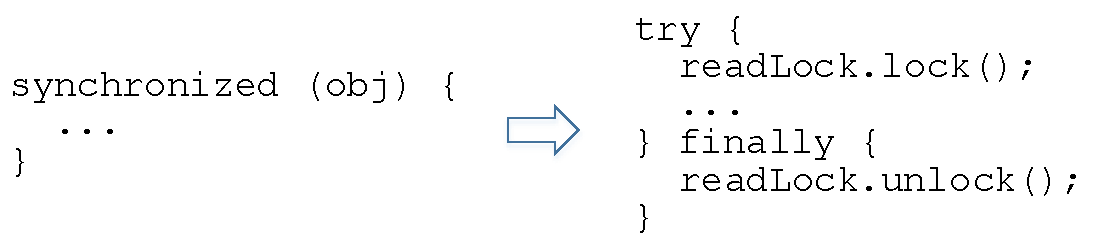
\includegraphics[scale=0.35]{pattern1}&4\\\hline
%		Changing lock instance&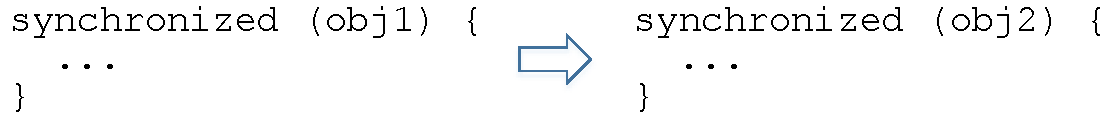
\includegraphics[scale=0.35]{pattern2}&6\\\hline
%		Changing critical section&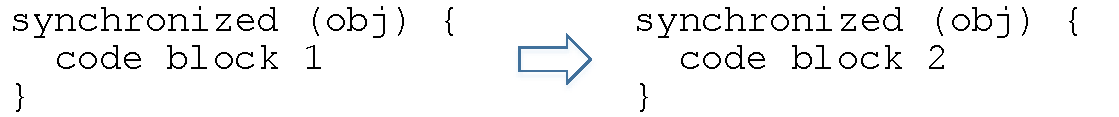
\includegraphics[scale=0.35]{pattern3}&35\\\hline
%		Adding or removing \texttt{volatile}&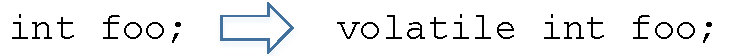
\includegraphics[scale=0.35]{pattern4}&47\\\hline
%		Thread-safe class replacement&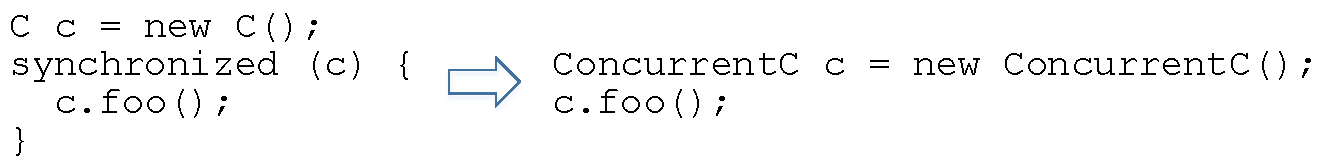
\includegraphics[scale=0.35]{pattern5}&32\\\hline
%		Thread management&&\\\hline
%		%Other class replacement&Some other concurrent related class replacement&\\\hline
%	\end{tabular}
%\end{table*}

%Switch to another type of lock
%Switch to another lock instace
%Change critical sections, which are protected by synchronization
%Add or remove 'volatile' modifier of a class field
%Use thread-safe class instead of handling concurrency control manually

%Table~\ref{} and \ref{} show an overview of our extracted change patterns. \zhong{Please explain the columns.}

Table~\ref{table:patterns} and Table~\ref{table:patterns2} show an overview of our extracted change patterns. The first column is the sequence number of patterns. The ``source'' column shows the concrete examples of patterns. We put related source code in it. The left is the original code and the right is the modified code. We align the corresponding statements. We use different colors to mark modified lines. The ``pattern'' column shows the extracted patterns. They are short as they ignore the specific statements.

\begin{table*}
	\centering
\caption{Change patterns}\vspace*{-3ex}
	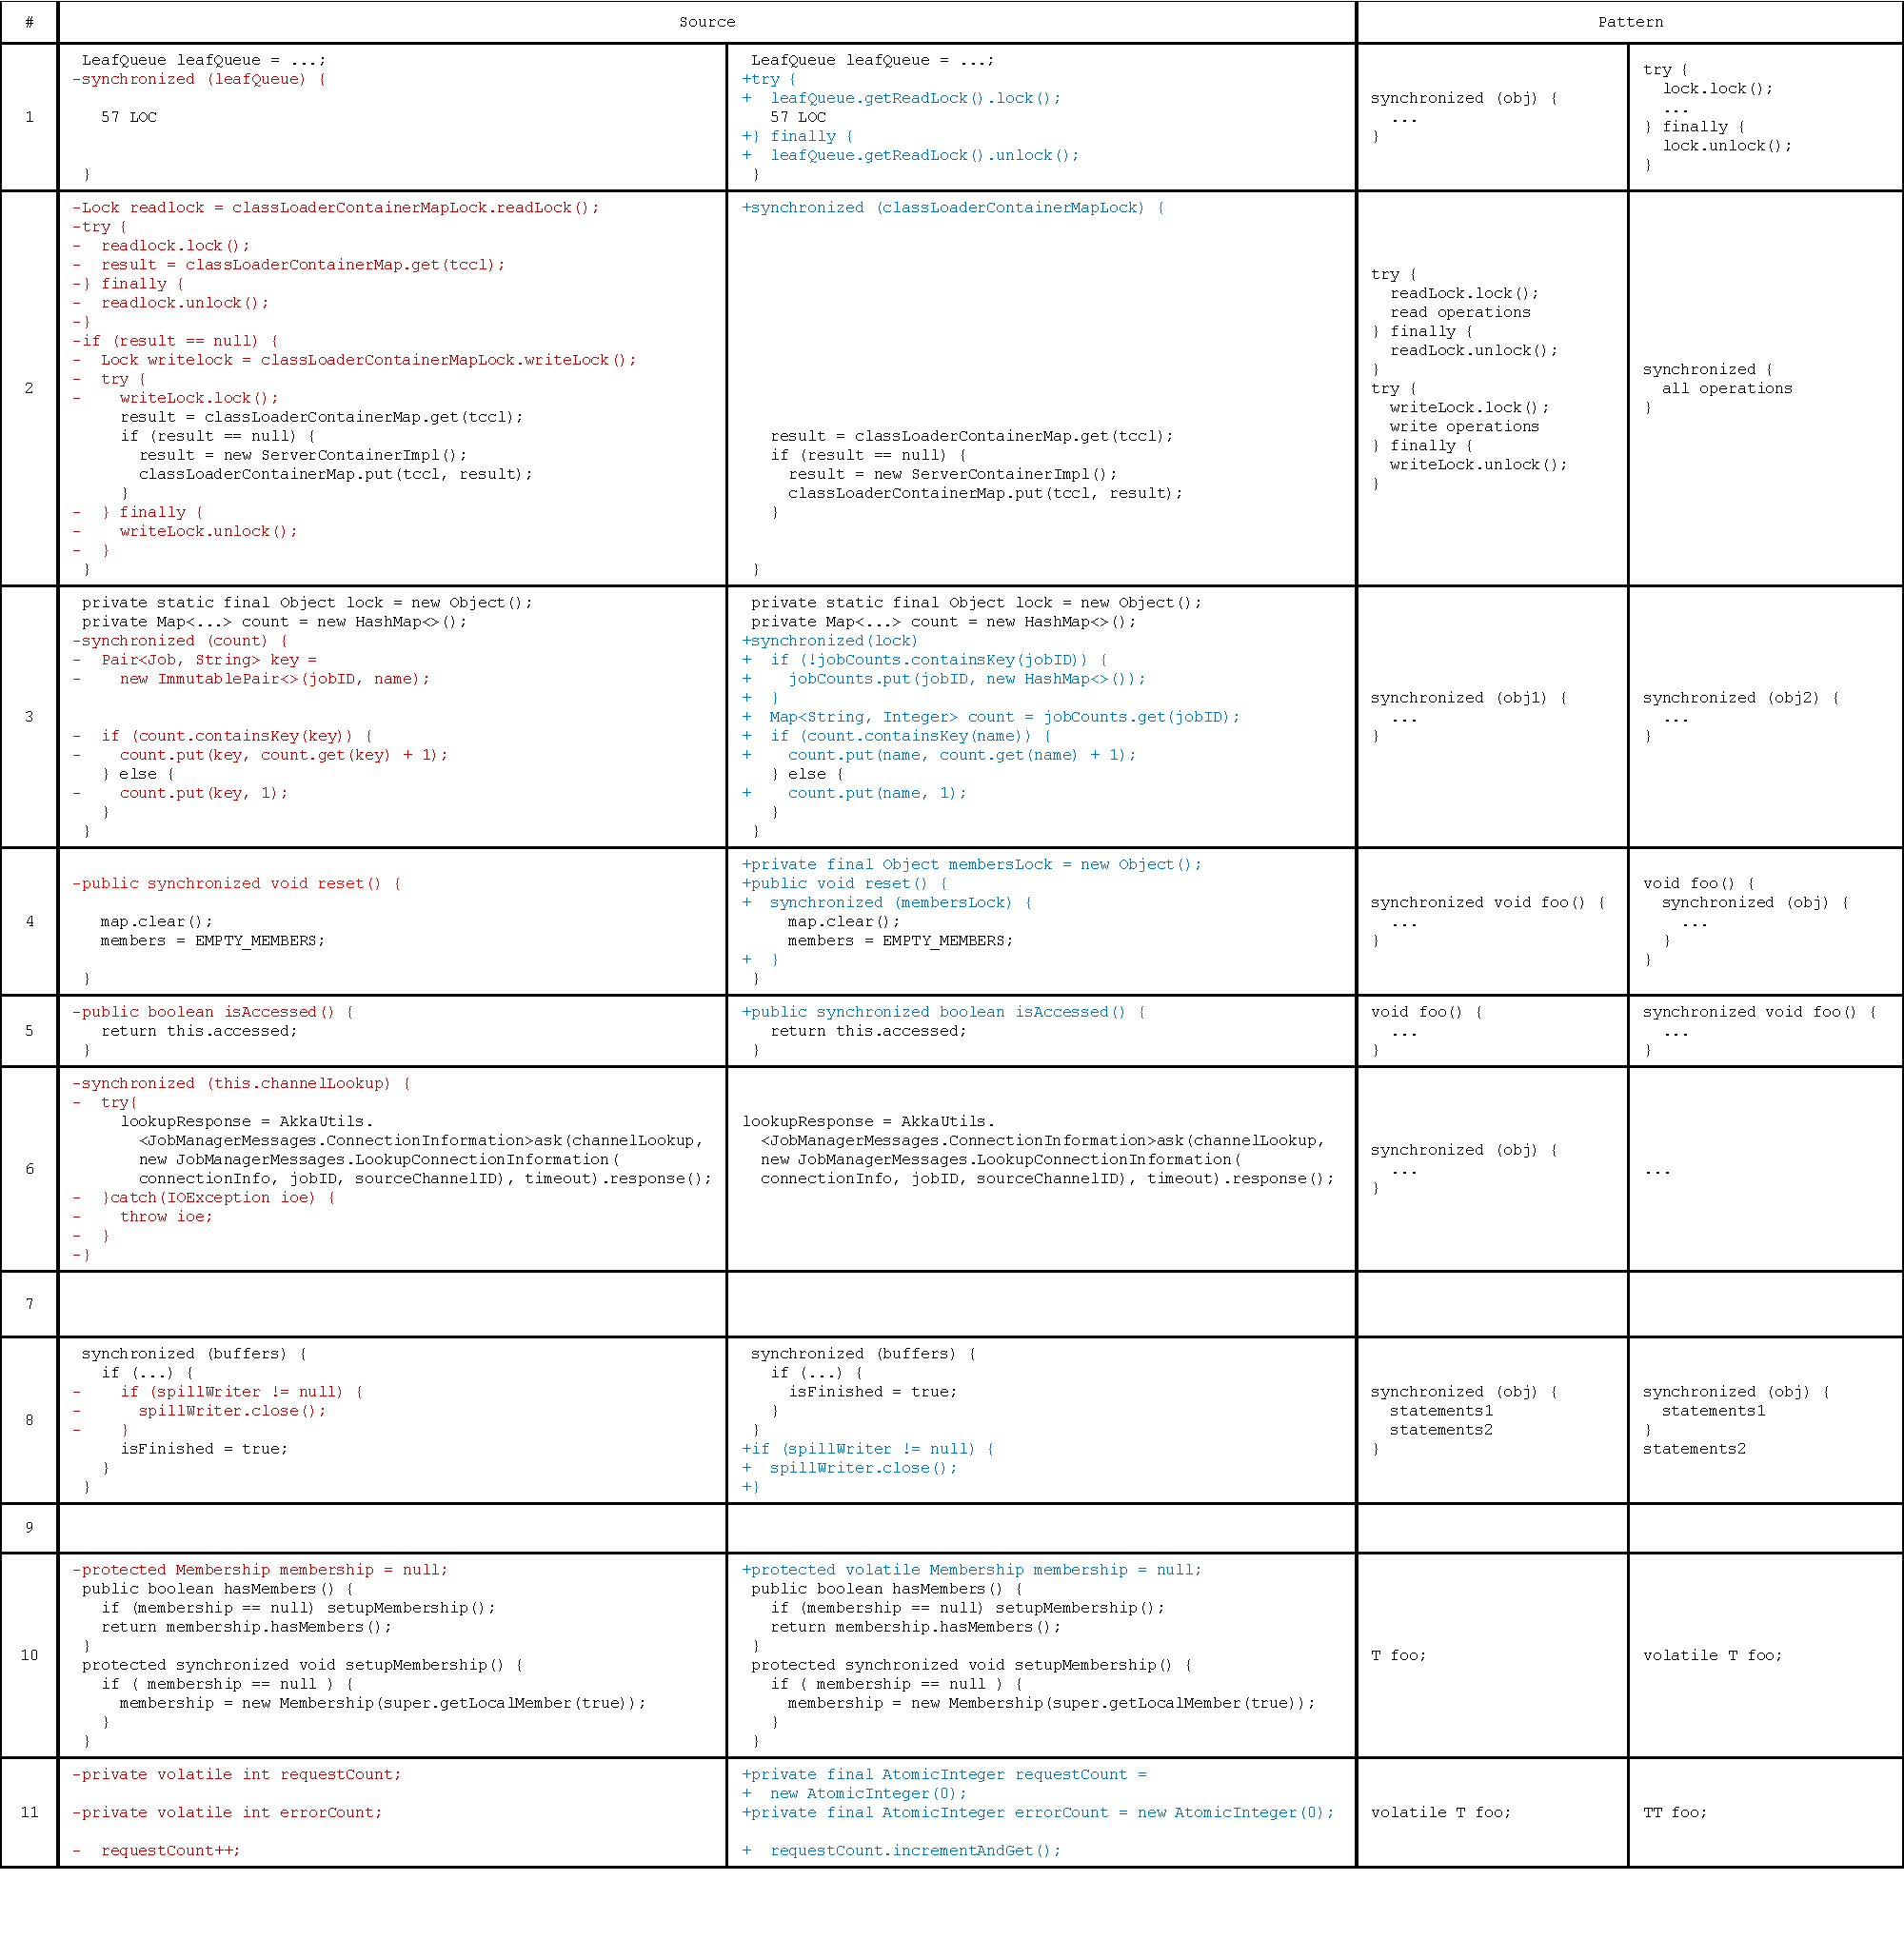
\includegraphics[width=1\textwidth]{patterns}	
	\label{table:patterns}\vspace*{-3ex}

\end{table*}
\begin{table*}
	\centering
	\caption{Change patterns (Cont.)}\vspace*{-3ex}
	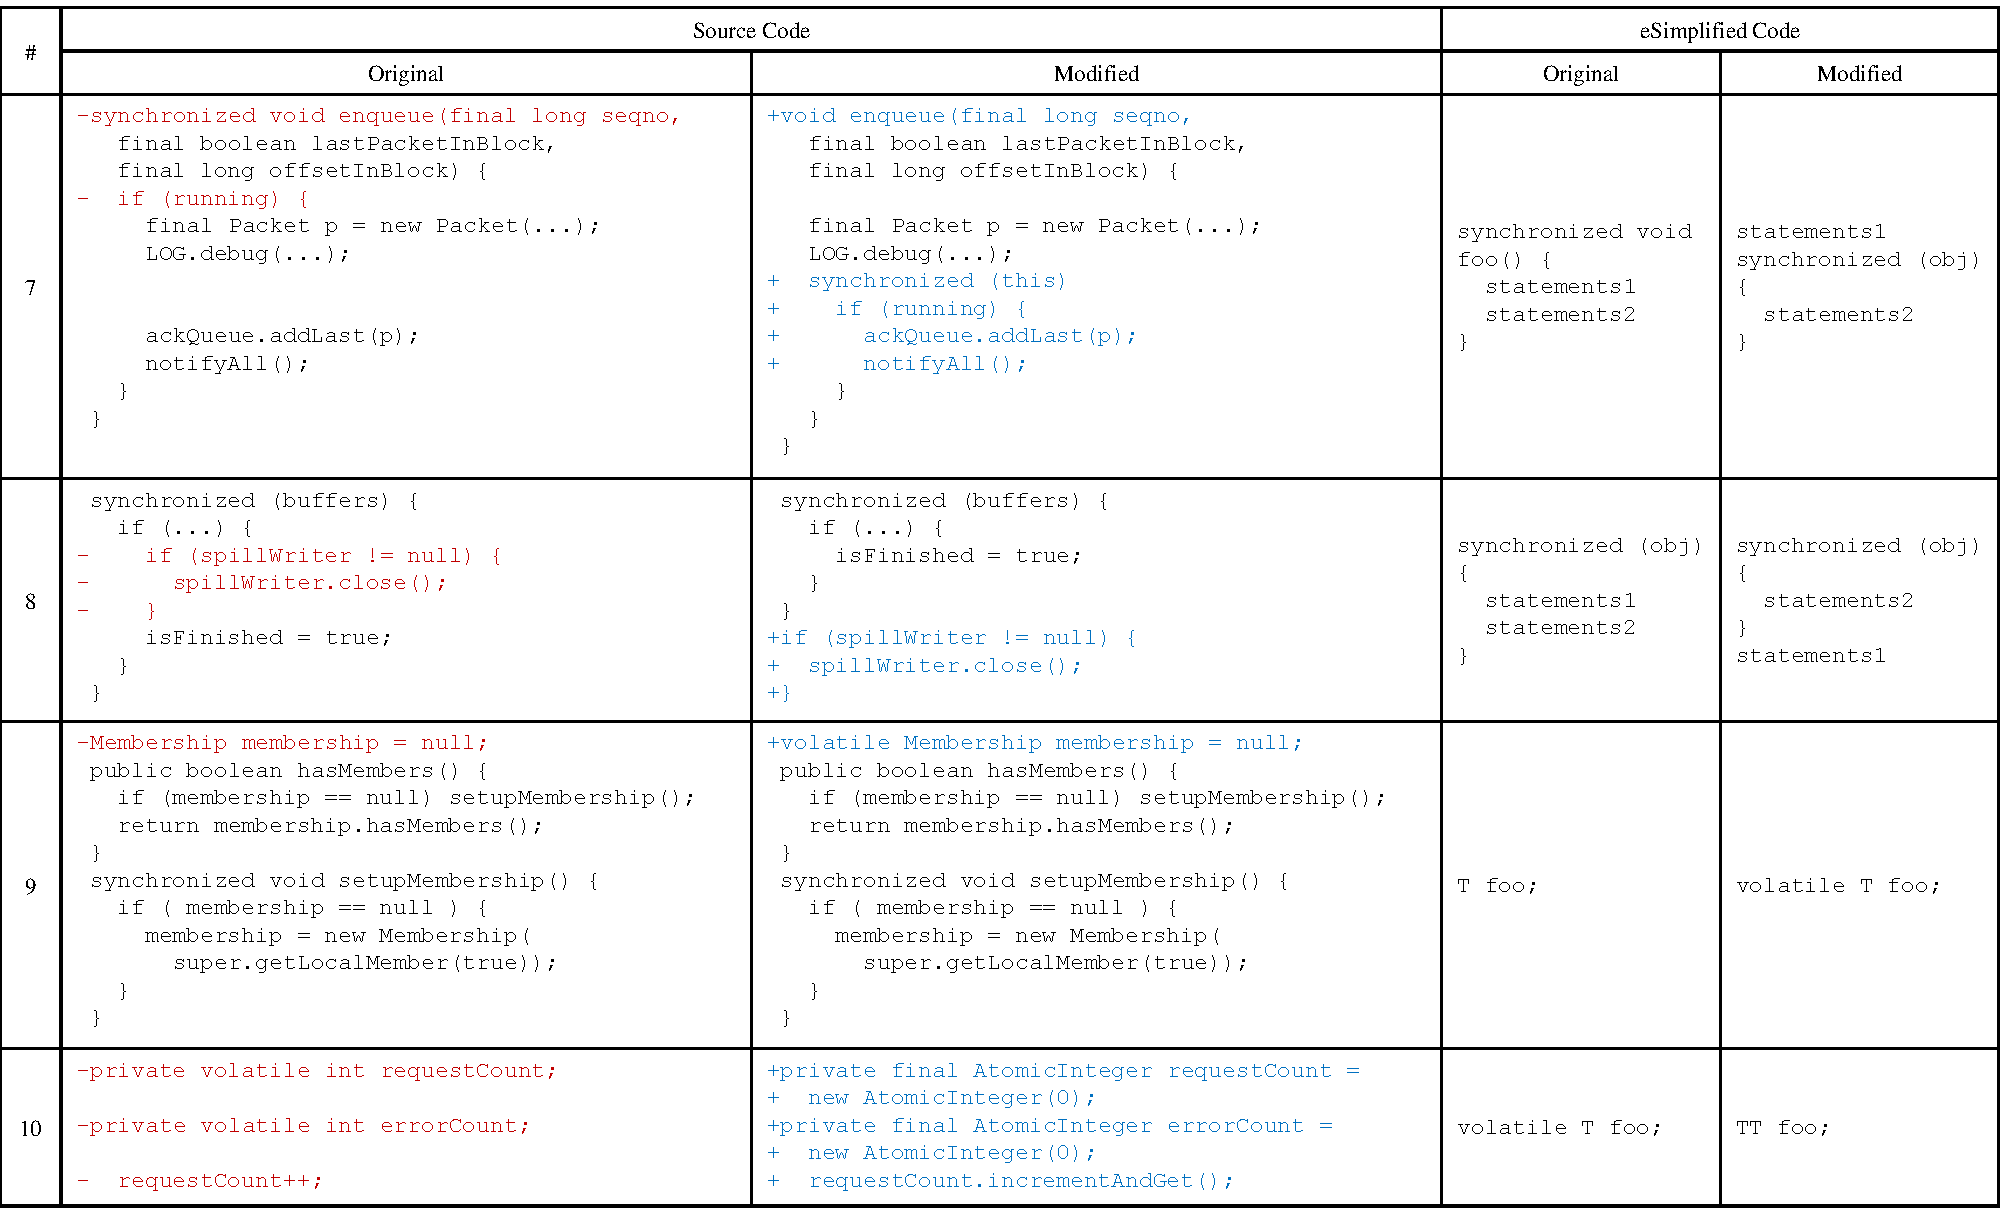
\includegraphics[width=1\textwidth]{patterns2}
	\label{table:patterns2}\vspace*{-3ex}
\end{table*}
\noindent
\textbf{1. Changing lock types.} It is feasible to lock resources with different mechanisms. For example, Java has a keyword, \CodeIn{synchronized}. The keyword can lock a block of code lines. With the keyword, programmers do not have to acquire and release resources explicitly. Alternatively, programmers can explicitly lock resources with APIs (\emph{e.g.}, \CodeIn{ReentrantLock}). Explicit locks offer more features than the \CodeIn{synchronized} keyword does. For example, with such APIs, programmers can determine the conditions for a lock. As another example, besides exclusive locks, programmers can use shared locks. When a thread is holding an exclusive lock, other threads have to wait until it is released. In contrast, shared locks allow multiple threads to hold the lock with specific actions. For example, \CodeIn{ReadWriteLock} allows multiple read actions, but denies multiple write actions.%\zhong{Please explain what exclusive and shared locks are, and their benefits.}

%ReentrantLock, ReentrantReadWriteLock, StampedLock are all API level locks in Java. Although 'synchronized' keyword is convenient and straightforward, we need other locks when we have more requirements. ReentrantLock is a reentrant lock, which means a lock can be acquired repeatedly in the same thread. It is a exclusive lock with the similar behaviour as monitor lock but has more features such as fairness, condition and tryLock. ReadWriteLock is a pair of locks, which allows concurrent access to read operations when there is no write operation going on but exclusive access to write operations. StampedLock is a lock which provides three modes, namely writing, reading and optimistic reading. This lock is usually used in design of thread-safe classes.
%Programmers can change their lock types due to various considerations. For example, the \CodeIn{synchronized} keyword can fail to satisfy fairness (\zhong{What is fairness? Why does it matter?}), programmers have to change such implicit locks to explicit locks. \zhong{Add an example for each situation.}

We find that programmers can replace the \CodeIn{synchronized} keyword with parallel API classes. For example, the first item of Table~\ref{table:patterns} comes from YARN-5825\footnote{\url{https://issues.apache.org/jira/browse/YARN-5825} To save space, we remove the URLs of the other Apache issues. Their URLs can be built by replacing the above URL with their issue number.}. To improve the performance, programmers replaced the \CodeIn{synchronized} with the \CodeIn{getReadLock} method. The method returns a shared lock, so multiple threads can read the query simultaneously.

%3e4b1ae6dc786b268505aa2e64067432519c2bcf
%\begin{figure*}
%	\centering
%	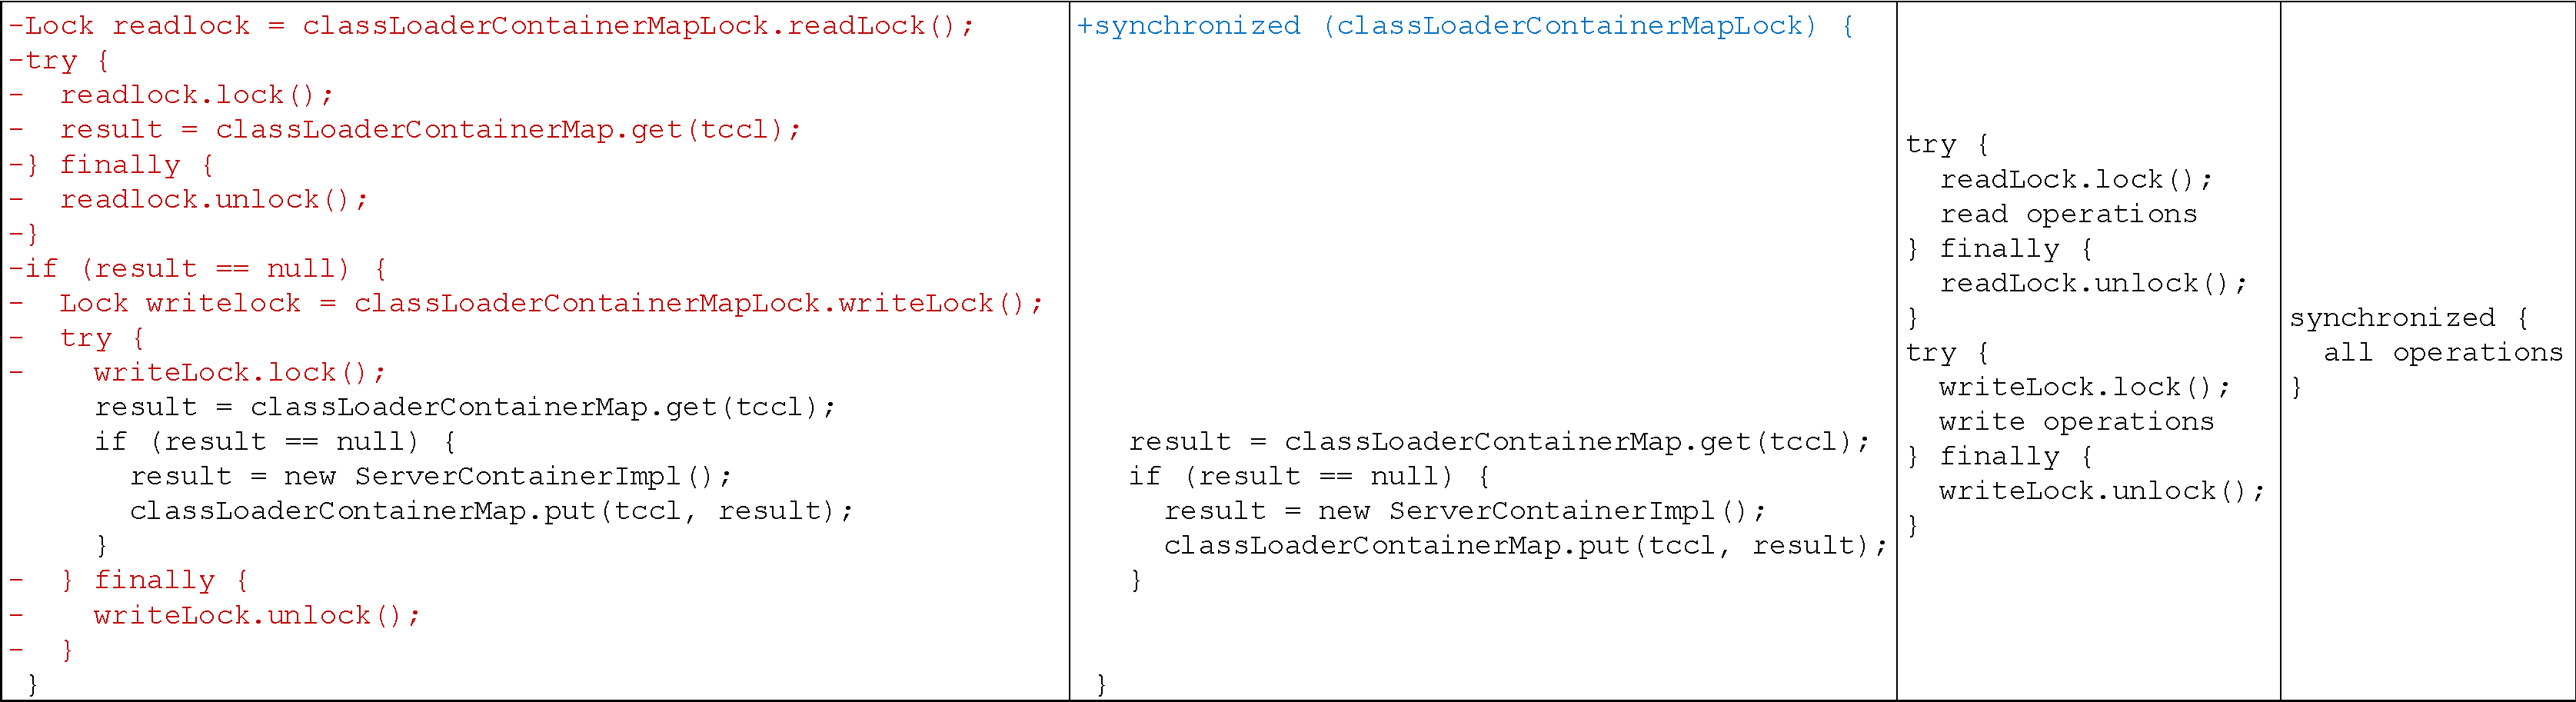
\includegraphics[scale=0.3]{locktype2}
%	\caption{Example 2}
%\zhong{It may be better, if you merge the example figures into a table like Table 1.}
%\end{figure*}

%\zhong{Please replace all texttt with CodeIn.}

%They also might switch to a reader-writer lock \cite{journals/cacm/CouroisHP71} from a normal lock to improve concurrency when there are plenty of concurrent read operations. Here are some examples. \zhong{add an example for this.}
Meanwhile, we find that programmers can replace parallel API classes with the \CodeIn{synchronized} keyword. For example, the second item of Table~\ref{table:patterns} comes from Tomcat\footnote{\url{https://svn.apache.org/viewvc?view=revision&revision=1414150}}. This commit is not reported, and we find it through our SVM classifier.% \zhong{List the commit message/log}.

%3e4b1ae6dc786b268505aa2e64067432519c2bcf
\begin{lstlisting}
A ReadWriteLock cannot be used to guard a WeakHashMap. The WeakHashMap may modify itself on get(), as it processes the reference queue of items removed by GC. Either a plain old lock / synchronization is needed, or some other solution.
\end{lstlisting}

As the above message explains, a developer complained that the \CodeIn{ReadWriteLock} method does not guard the \CodeIn{WeakHashMap} variable, since the \CodeIn{get()} method can modify the \CodeIn{WeakHashMap} variable, and the modification can bypass the lock. In this example, programmers fixed the problem by replacing the methods with the \CodeIn{synchronized} keyword.%todo more detail

%When they find that they only need a simple exclusive lock, they switch to synchronized block. \zhong{add an example for this}
%\begin{figure}
%	\centering
%	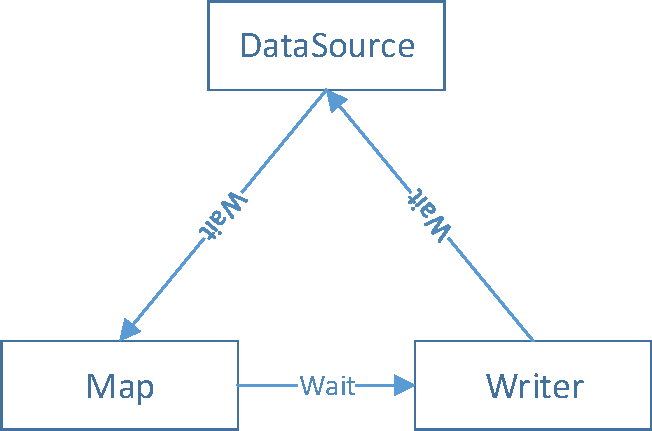
\includegraphics[height=1.7in]{deadlock}
%	\caption{Deadlock}
%	\label{figure:deadlock}
%%\zhong{Please add resource columns and add edges to denote resource manipulations.}
%\end{figure}

\noindent
\textbf{2. Changing locked variables.} A program needs to lock variables before it enters critical section bodies. During software maintenance, programmers can change locked variables, and we find that the main purpose is to repair bugs. For example, the third item of Table~\ref{table:patterns} comes from FLINK-1419. This bug complains that \CodeIn{DistributedCache} does not preserve files for subsequent operations. Based on its discussions, we understand that in the buggy file, programmers lock \CodeIn{count}, while they shall lock \CodeIn{lock}. To fully fix the bug, programmers also modified the critical sections and the \CodeIn{finally} clause.

As another example, when repairing bugs, programmers can add new locks. For example, the fourth item of Table~\ref{table:patterns} comes from Tomcat\footnote{\url{https://bz.apache.org/bugzilla/show\_bug.cgi?id=58386}}. It includes the following message:

\begin{lstlisting}
Reported by RV-Predict (a dynamic race detector) when running the test suite:
Data race on field org.apache.catalina.tribes.io.ObjectReader.accessed: {{{
Concurrent write in thread T93 (locks held: {...})
\end{lstlisting}

The data race indicates that the \CodeIn{isAccessed()} is not locked, so programmers add the \CodeIn{synchronized} keyword to allow locking on the method.


We find that programmers can also delete unnecessary locks. For example, the fifth item of Table~\ref{table:patterns} comes from Flink:

\begin{lstlisting}
...Remove synchronized blcok in getReceiverList of ChannelManager which effectively serialized the connection lookup calls of a single task manager.
\end{lstlisting}
%\zhong{show the URL of the commit}.
%\zhong{show what programmers say. Why it is unnecessary}.

As the above commit messages says, programmers removed synchronization from the \CodeIn{ChannelManager} class to improve the performance.


%\zhong{show the URL of the commit}.
%\zhong{show what programmers say. Why it is unnecessary}.




%\zhong{Why do you present the above stack trace.}

%\zhong{Instead of why a deadlock occurs, you shall explain why the modification in Table~\ref{table:patterns2} repaired the deadlock. If the modification alone is insufficient, add more details here.}
%As shown in Figure~\ref{figure:deadlock}, a deadlock can occur when three threads execute in a specific order. Here, we use $s1$ and $s2$ to denote two statements. An arrow from $s1$ to $s2$ means $s1$ cannot be returned before $s2$ has been returned. The \CodeIn{DataSource} (thread-1) is waiting to be notified by the \CodeIn{Writer} (thread-2) when holding lock A. The \CodeIn{Writer} (thread-2) is trying to acquire lock B. But lock B is held by the \CodeIn{Map} (thread-3). And the \CodeIn{Map} (thread-3) is trying to acquire lock A, which is held by the \CodeIn{DataSource} (thread-1). Here is a waiting chain. This is a kind of bug known as deadlock. The problem is that the \CodeIn{DataSource} (thread-1) does not need to hold lock A while waiting to be notified. So the developer removed the unnecessary synchronization.

%f0e627bb8c9daedb3b064027cac37ce4849bab64
In some other cases, we find that programmers can refine their locked resources to improve performance. For example, the seventh item of Table~\ref{table:patterns} comes from Tomcat\footnote{\url{https://bz.apache.org/bugzilla/show_bug.cgi?id=58382}}. The original code locks the instance of a class, but the modified code locks only the \CodeIn{membersLock} field.

\noindent
\textbf{3. Modifications inside critical section bodies.} A critical section is a code block that is executed, when a thread locks the corresponding resources. We notice that even modifications inside critical section bodies can repair concurrency bugs. For example, the sixth item of Table~\ref{table:patterns2} comes from FLINK-2384. It is caused by an implicit lock in the \CodeIn{spillWriter.close()} method. As programmers typically do not known such locks inside APIs, the lock leads to the deadlock. Indeed, we find that a recent benchmark~\cite{lin2015ase} includes a similar concurrency bug, and Lin \emph{et al.}~\cite{lin2016lockpeeker} proposed an approach that detects such implicit locks inside APIs. In this example, programmers move the \CodeIn{spillWriter.close()} method outside the critical section body to resolve the deadlock.

%
%\begin{lstlisting}
%"CHAIN DataSource (at createInput(ExecutionEnvironment.java:502) (org.apache.flink.api.java.hadoop.mapreduce.HadoopInputFormat)) -> FlatMap (FlatMap at readFlinkTuplesFromThriftParquet(ParquetThriftEntitons.java:96)) (7/8)" daemon prio=10 tid=0x00007f934005b000 nid=0x73c4 in Object.wait() [0x00007f93c16ac000]
%java.lang.Thread.State: TIMED_WAITING (on object monitor)
%
%"IOManager writer thread #1" daemon prio=10 tid=0x00007f93d8b7b000 nid=0x73a8 waiting for monitor entry [0x00007f93c2fc5000]
%java.lang.Thread.State: BLOCKED (on object monitor)
%
%"Map (Projection [0, 1, 2, 3, 4]) (7/8)" daemon prio=10 tid=0x00007f92b0434800 nid=0x74a3 waiting for monitor entry [0x00007f93a32f1000]
%java.lang.Thread.State: BLOCKED (on object monitor)
%\end{lstlisting}

%<<<<<<< HEAD
%f0e627bb8c9daedb3b064027cac37ce4849bab64
%In some other cases, we find that programmers can refine their locked resources to improve performance. For example, the seventh item of Table~\ref{table:patterns} comes from Tomcat\footnote{\url{https://bz.apache.org/bugzilla/show_bug.cgi?id=58382}}. The original code locks the instance of a class, but the modified code locks only the \CodeIn{membersLock} field.

%\noindent
%\textbf{3. Modifications on critical section bodies.} A critical section is a code block that is executed, when a thread locked the corresponding resources. The modifications on critical section bodies indicate new functionalities or refactoring. For example, the eighth item of Table~\ref{table:patterns2} comes from HDFS-4200. To reduce the size of a critical section body, programmers refactor the body into several methods. Indeed, this issue involves modifications that are related to even more change patterns (\emph{e.g.}, adding locked variables).
%=======
Besides the above example, the majority of modifications on critical section bodies indicates new functionalities or refactoring. For example, the eighth item of Table~\ref{table:patterns2} comes from HDFS-4200. To reduce the size of a critical section body, programmers refactor the body into several methods. Indeed, this issue involves modifications that are related to even more change patterns (\emph{e.g.}, adding locked variables).
%>>>>>>> 9e8b767a2cf136027178c18c50d9c5eea616e630

%c93d9eaf363a535dff25cc4e7db400d879e73bb1
%Add option to use single actor system for local execution. Use local connection manager if a single task manager is used for local execution. Remove synchronized blcok in getReceiverList of ChannelManager which effectively serialized the connection lookup calls of a single task manager.
%\zhong{Why do you list the following commits? If you cannot list the following commit in Table~\ref{table:patterns2}, split it into the original code and fixed code. Explain them separatively.}

%Modifications on statements change statements of critical sections.

%efca79cfb7b496b4bec70561cc94af069c644ef2
%[FLINK-2384] [runtime] Move blocking I/O call outside of synchronized block
%Problem: Waiting on asynchronous write requests with the partition lock can
%result in a deadlock, because all other operations on the same partition are
%blocked. It is possible that the I/O writer itself needs to access the
%partition, in which cases the whole program blocks.
%Solution: Move the wait outside the synchronized block. This was not necessary
%before, because no operation assumes the spilling to be finished when the
%finish call has returned.




%Modifications on locked resources change the criteria of entering critical sections.  \zhong{Please check whether the samples explain the corresponding situations.}



%Example 9.



\noindent
\textbf{4. Changing the \CodeIn{volatile} keyword.} In Java, the \CodeIn{volatile} keyword denotes a variable that is saved in the main memory. For a \CodeIn{volatile} variable, a thread reads its latest value from the main memory, instead of the obsolete  value in the cache. Although it can improve the overall performance, races can occur, when multiple threads read and write \CodeIn{volatile} variables simultaneously.

%8313fa0f1ca277e9633a78f461804abc3c5515b8
%Fix https://bz.apache.org/bugzilla/show_bug.cgi?id=58392
%Double-checked locking needs to use volatile to be thread-safe
We find that programmers can add the \CodeIn{volatile} keyword to improve performance. For example, the ninth item of Table~\ref{table:patterns2} comes from Tomcat\footnote{\url{https://bz.apache.org/bugzilla/show_bug.cgi?id=58392}}. It reports a data race, and the bug was repaired by adding the \CodeIn{volatile} keyword.

%560cd00890b3f6af2aca0c3a9d51a45f880692dd
%Fix a FindBugs warning (increment of volatile not atomic)

%\zhong{Please explain why you need two samples for this situation.}
Besides adding the keyword, we find that programmers have to remove the \CodeIn{volatile} keyword, since they do not fully understand its meanings. For example, in tenth item of Table~\ref{table:patterns2} comes from Tomcat\footnote{\url{https://svn.apache.org/viewvc?view=revision&revision=1360946}}. In this bug, programmers auto-increment a \CodeIn{volatile} variable, but such an action is not atomic. As a result, FindBugs reports it as a bug, and programmers have to remove the keyword.

\noindent
\textbf{5. Replacing self-written code with Parallel APIs.} Programmers can implement concurrent code by themselves, but later they realize that it is easier to call APIs that already implement their functionalities. For example, a previous version of Hadoop has the following code:% \zhong{Replace the below commit with the buggy code.}


\begin{lstlisting}
private volatile long genstamp;
public synchronized long nextStamp() {
  this.genstamp++;
  return this.genstamp; }
\end{lstlisting}

Later, a programmer realized that it is better to replace the above code with the \CodeIn{AtomicLong} class. He reported the issue (HDFS-4029), and set its priority as major. Here, \CodeIn{AtomicLong} is a thread-safe version of type long. It allows updating a \CodeIn{Long} value without explicit synchronization and it is fast.

%It not only offers a simple interface, but also has a different implementation than the example code above. It uses \CodeIn{Unsafe} class, which provides unsafe operations as its name represents. This class allows low-level programming in Java, which is considered unsafe but can save running time without the check to guarantee safety. It might be promoted to be public API in Java 9. The fixed code is as follow:

%\zhong{Replace the below commit with the fixed code.}

\begin{lstlisting}
private volatile long genstamp;
public long nextStamp() {
  return genstamp.incrementAndGet(); }
\end{lstlisting}

Besides replacing directly, programmers can replace their code with parallel APIs that implement similar functions. For example, the below code comes from LUCENE-2779:

\begin{lstlisting}
protected ... fileMap = new HashMap<...>();
public final boolean fileExists(String name) {
  ensureOpen();
  RAMFile file;
  synchronized (this) {
    file = fileMap.get(name);
  }
  return file != null; }
\end{lstlisting}

Instead of handling synchronization by themselves, programmers replaced the above code with a parallel API:

\begin{lstlisting}
protected ... fileMap = new ConcurrentHashMap<...>();
public final boolean fileExists(String name) {
  ensureOpen();
  return fileMap.containsKey(name); }
\end{lstlisting}

%\textbf{Other class replace}
%
%\textbf{Thread resource management}
%
%When we do concurrent programming, we need to pay attention to resource management such as threads, locks.
%
%Thread management is to deal with the management of thread-related resources.
%
%\textbf{Thread sleep wait notify}
%
%It is a another way of synchronization which is less common than locking.
%
%\textbf{Final in multiple threads}

In summary, in our study, we identify five types of change patterns in total. First, we find that programmers can modify parallel keywords and locked variables, and such modifications are mainly for repairing bugs and improving performance. Second, we notice modifications on critical section bodies, and such modifications often indicate new functions. Finally, we notice that self-written code is replaced with corresponding parallel APIs. In most cases, we find that maintaining concurrent code is not a one-direction migration. For example, there are several different ways to implement a lock. Programmers shall carefully analyze their programming contexts to determine which is their best choice. As shown in our examples, during software maintenance, programmers can migrate to any types according to their need.

\subsection{RQ2. The usefulness of our change patterns.}
\label{sec:result:sample}

%\zhong{Try to add an example for each change pattern.}
%\zhong{How many pull requests did you submit?}

In total, we made three pull requests. We made the first pull request on Schmince-2\footnote{\url{https://github.com/derekmu/Schmince-2}}. This is a game, where players control space tourists for adventure. It has the following code:

\begin{lstlisting}
public class DRandom {
  private ... random = new ThreadLocal<Random>() {
    protected Random initialValue() {
      return new Random();
    }
  };
  public static Random get() {
    return random.get();
  }
}
\end{lstlisting}

The above code implements a class that generates random values for multiple threads. We find that J2SE provides the \CodeIn{ThreadLocalRandom} class\footnote{\url{https://docs.oracle.com/javase/8/docs/api/java/util/concurrent/ThreadLocalRandom.html}} that implements the identical function. According to our fifth change pattern, we made a pull request to replace the above code with the corresponding API\footnote{\url{https://github.com/derekmu/Schmince-2/pull/1}}. This pull request is already confirmed.
%\begin{lstlisting}
%+import java.util.concurrent.ThreadLocalRandom;
%public class DRandom {
%-    private static ThreadLocal<Random> random = new ThreadLocal<Random>() {
%-        protected Random initialValue() {
%-            return new Random();
%-        }
%-    };
%public static Random get() {
%-        return random.get();
%+        ThreadLocalRandom.current();
%}
%}
%\end{lstlisting}

%This example shows a change from ThreadLocal$<$Random$>$ to ThreadLocalRandom from JDK7. It is from a Schmince-2, a game on Google Play. We make the change and our pull request\footnote{\url{https://github.com/derekmu/Schmince-2/pull/1}} has been accept. ThreadLocalRandom should be used when available in place of ThreadLocal$<$Random$>$. For JDK7 the difference is minimal, but JDK8 starts including optimizations for ThreadLocalRandom. The ThreadLocal class provides thread-local variables. The ThreadLocalRandom class is a random number generator isolated to the current thread.
\begin{figure*}
	\centering
	\subfigure[Ascending-high]{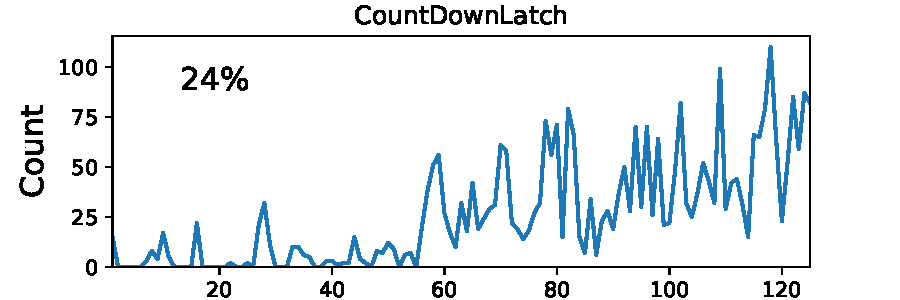
\includegraphics[width=2.3in]{CountDownLatch}}
	\subfigure[Descending-high]{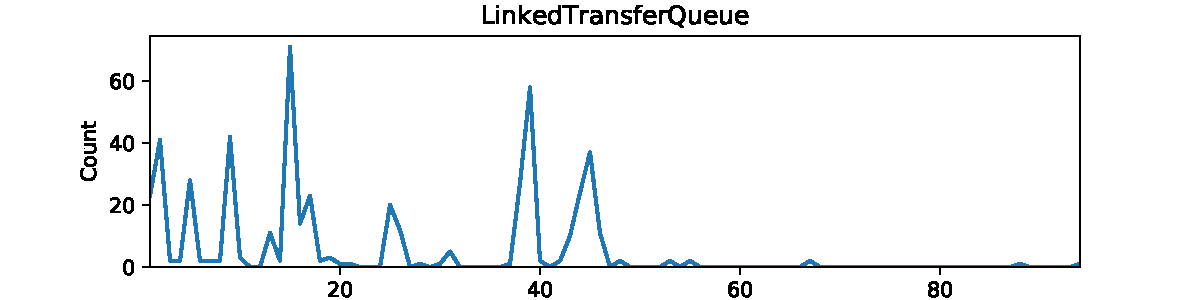
\includegraphics[width=2.3in]{LinkedTransferQueue}}
	\subfigure[Hybrid-high]{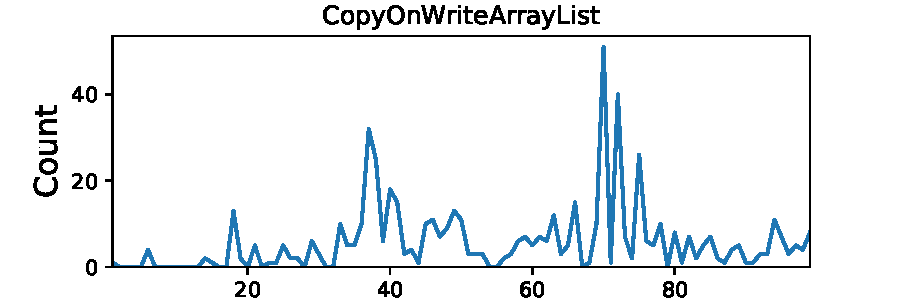
\includegraphics[width=2.3in]{CopyOnWriteArrayList}}
	
	\subfigure[Ascending-medium]{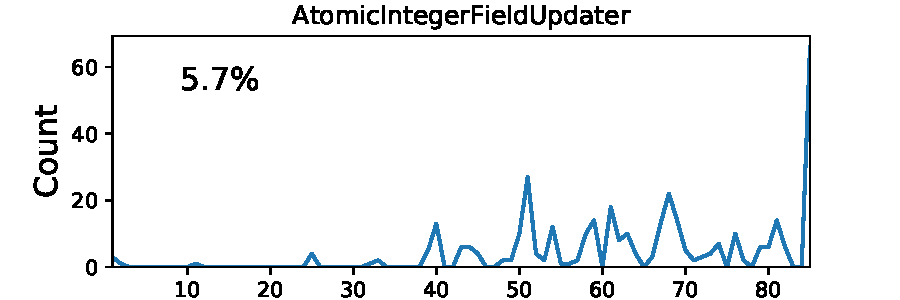
\includegraphics[width=2.3in]{AtomicIntegerFieldUpdater}}
	\subfigure[Descending-medium]{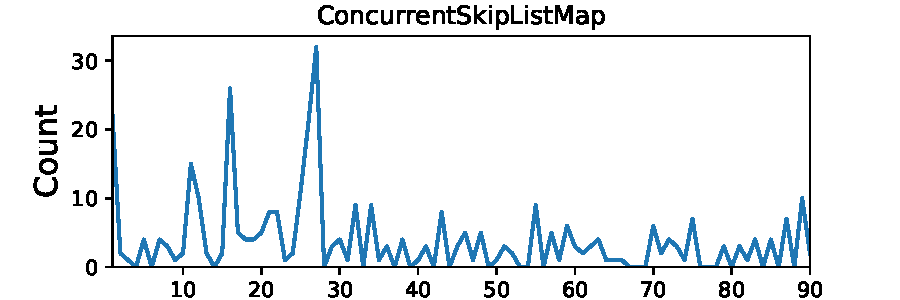
\includegraphics[width=2.3in]{ConcurrentSkipListMap}}
	\subfigure[Hybrid-medium]{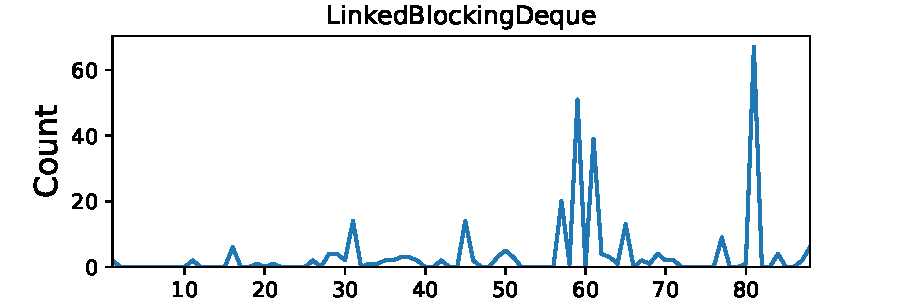
\includegraphics[width=2.3in]{LinkedBlockingDeque}}
	
	\subfigure[Ascending-low]{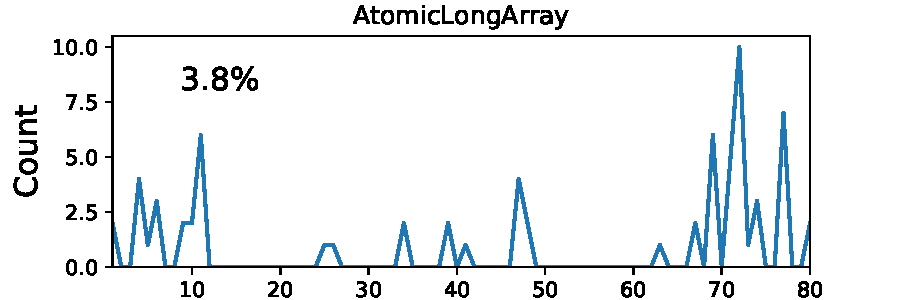
\includegraphics[width=2.3in]{AtomicLongArray}}
	\subfigure[Descending-low]{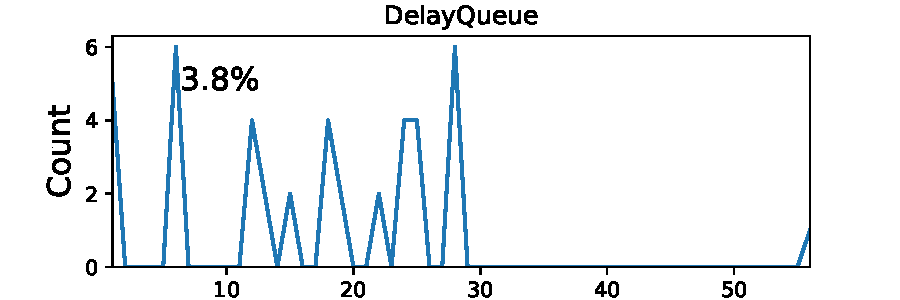
\includegraphics[width=2.3in]{DelayQueue}}
	\subfigure[Hybrid-low]{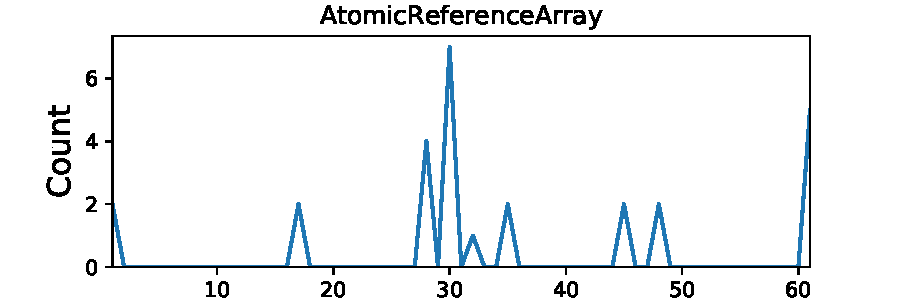
\includegraphics[width=2.3in]{AtomicReferenceArray}}
	
%	\subfigure[Descending]{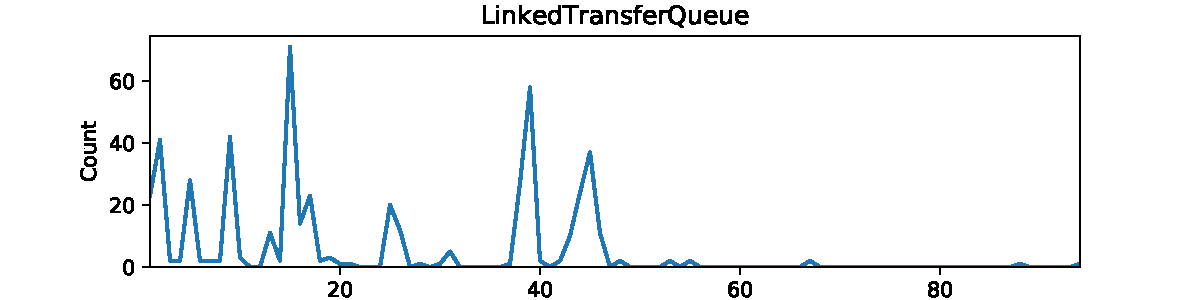
\includegraphics[width=2.3in]{LinkedTransferQueue}}
%	\subfigure[Hybrid]{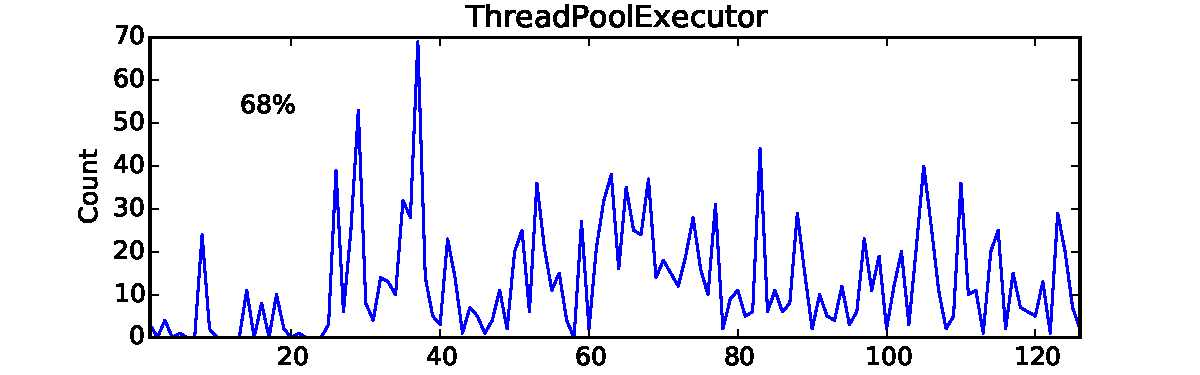
\includegraphics[width=2.3in]{ThreadPoolExecutor}}
%	\subfigure[High]{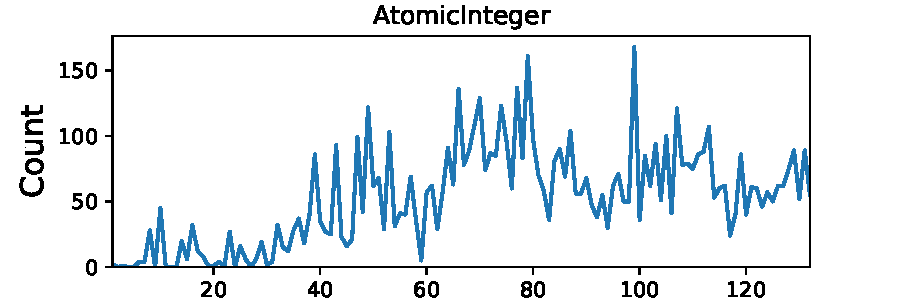
\includegraphics[width=2.3in]{AtomicInteger}}
%	\subfigure[Medium]{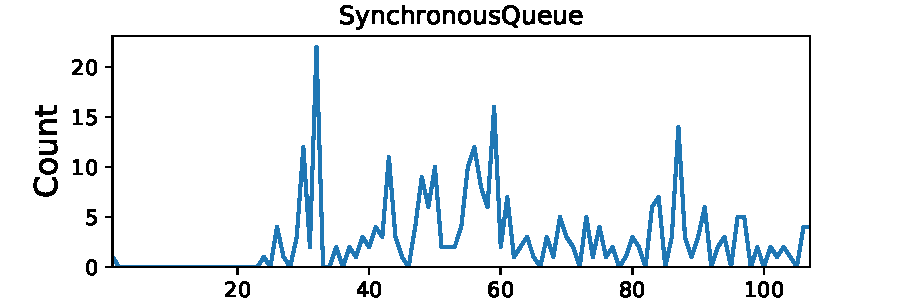
\includegraphics[width=2.3in]{SynchronousQueue}}
%	\subfigure[Low]{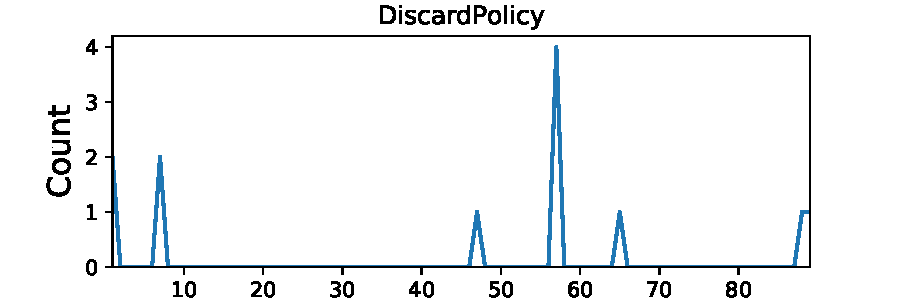
\includegraphics[width=2.3in]{DiscardPolicy}}
	\caption{Typical trends and their percents}
	\label{figure:trend}\vspace*{-3ex}
%\zhong{The labels shall be like ascending-high, ascending-medium, ascending-low, and etc. There shall be nine graphs in total. The percents of the nine graphs shall add up to 100\%.}
\end{figure*}
We made the second pull request on UnifiedEmail\footnote{\url{https://github.com/HexagonRom/android_packages_apps_UnifiedEmail}}. It is an Android email client. It has the following code:

\begin{lstlisting}
private static NotificationMap sActiveNotificationMap = null;
private static synchronized NotificationMap getNotificationMap(Context context) {
 if (sActiveNotificationMap == null) {
  sActiveNotificationMap = new NotificationMap();
  sActiveNotificationMap.loadNotificationMap(context);
 }
 return sActiveNotificationMap;
}
\end{lstlisting}

If the \CodeIn{sActiveNotificationMap} field is \CodeIn{null}, the above method creates a new map and assigns the new map to the field. To allow multiple threads to call the methods, programmers add the \CodeIn{synchronized} keyword to the method. We believe that when \CodeIn{sActiveNotificationMap} is not \CodeIn{null}, the lock is unnecessary, since it does not change the field. According to our second change pattern, we made the following modification to synchronize only the lines that modify the field:

\begin{lstlisting}
private static volatile NotificationMap sActiveNotificationMap = null;
private static NotificationMap getNotificationMap(Context context) {
  if (sActiveNotificationMap == null) {
    synchronized (NotificationUtils.class) {
      if (sActiveNotificationMap == null) {
       sActiveNotificationMap = new NotificationMap();
       sActiveNotificationMap.loadNotificationMap(context);
      }
    }
  }
  return sActiveNotificationMap;
}
\end{lstlisting}

%The above pull request is still pending.
The owner of the project deleted our pull request. We checked the pull requests of the project and found that there is no open or closed pull request. This project has more than 19,000 commits. It is possible that it has a strict policy of introducing external source code.

\begin{table}
	\centering
	\caption{Top 10 Active Classes}\vspace*{-2ex}
	\label{table:topapi}
	\begin{tabular}{|c|c|}\hline
		Class&Occurrence\\\hline
		AtomicInteger&6,891\\
		AtomicBoolean&4,180\\
		ConcurrentHashMap&3,976\\
		AtomicLong&3,926\\
		CountDownLatch&3,211\\
		AtomicReference&2,254\\
		Executors&2,026\\
		ThreadPoolExecutor&1,617\\
		LinkedBlockingQueue&1,553\\
		ConcurrentLinkedQueue&1,435\\\hline
	\end{tabular}\vspace*{-3ex}
\end{table}

We made the third pull request on Spider4java\footnote{\url{https://github.com/lichangshu/spider4java}}. It is a Java web crawler. It has the following code:

\begin{lstlisting}
public class Counter {
  protected int count;
  public Counter() {
    count = 0;
  }
  public synchronized void increment() {
    count = count + 1;
  }
  public synchronized int getValue() {
    return count;
  }
}
\end{lstlisting}

The above class implements a counter for multiple threads. As J2SE provides the identical API, \CodeIn{AtomicInteger}\footnote{\url{https://docs.oracle.com/javase/8/docs/api/java/util/concurrent/atomic/AtomicInteger.html}}, we modify it as follow:

\begin{lstlisting}
public class Counter {
  protected AtomicInteger count;
  public Counter() {
    count = new AtomicInteger();
  }
  public void increment() {
    count.getAndIncrement();
  }
  public int getValue() {
    return count.get();
  }
}
\end{lstlisting}
\begin{figure*}
	\centering
\subfigcapskip=-1ex
\subfigtopskip=-1ex
\captionsetup{aboveskip=0pt}
	\subfigure[Cassandra]{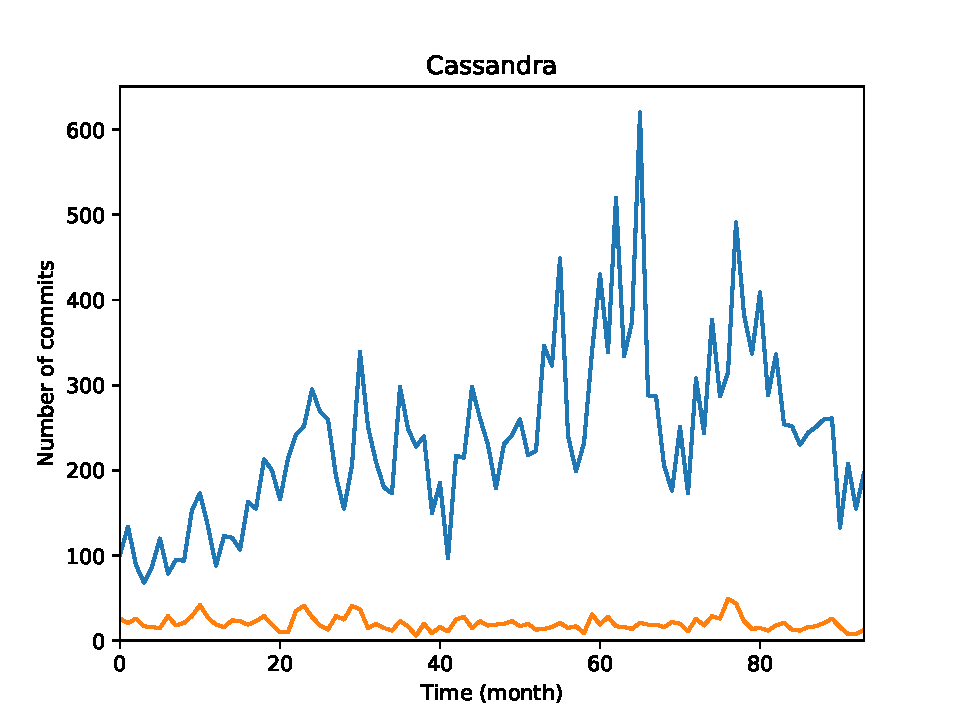
\includegraphics[height=1.4in]{cassandra}}
	\subfigure[Flink]{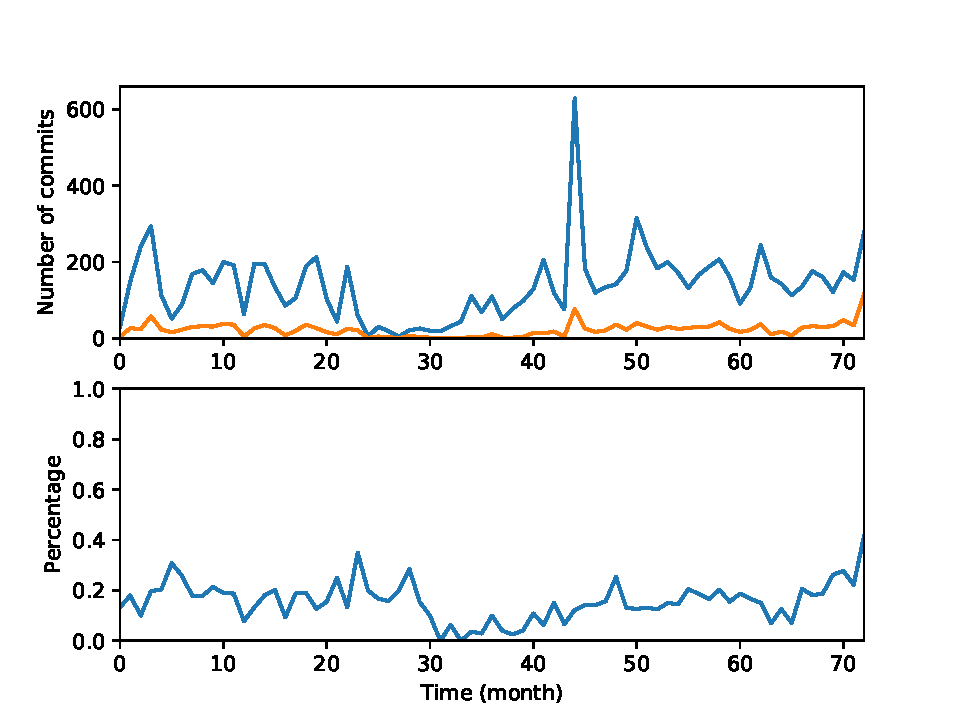
\includegraphics[height=1.4in]{flink}}
	\subfigure[Hadoop]{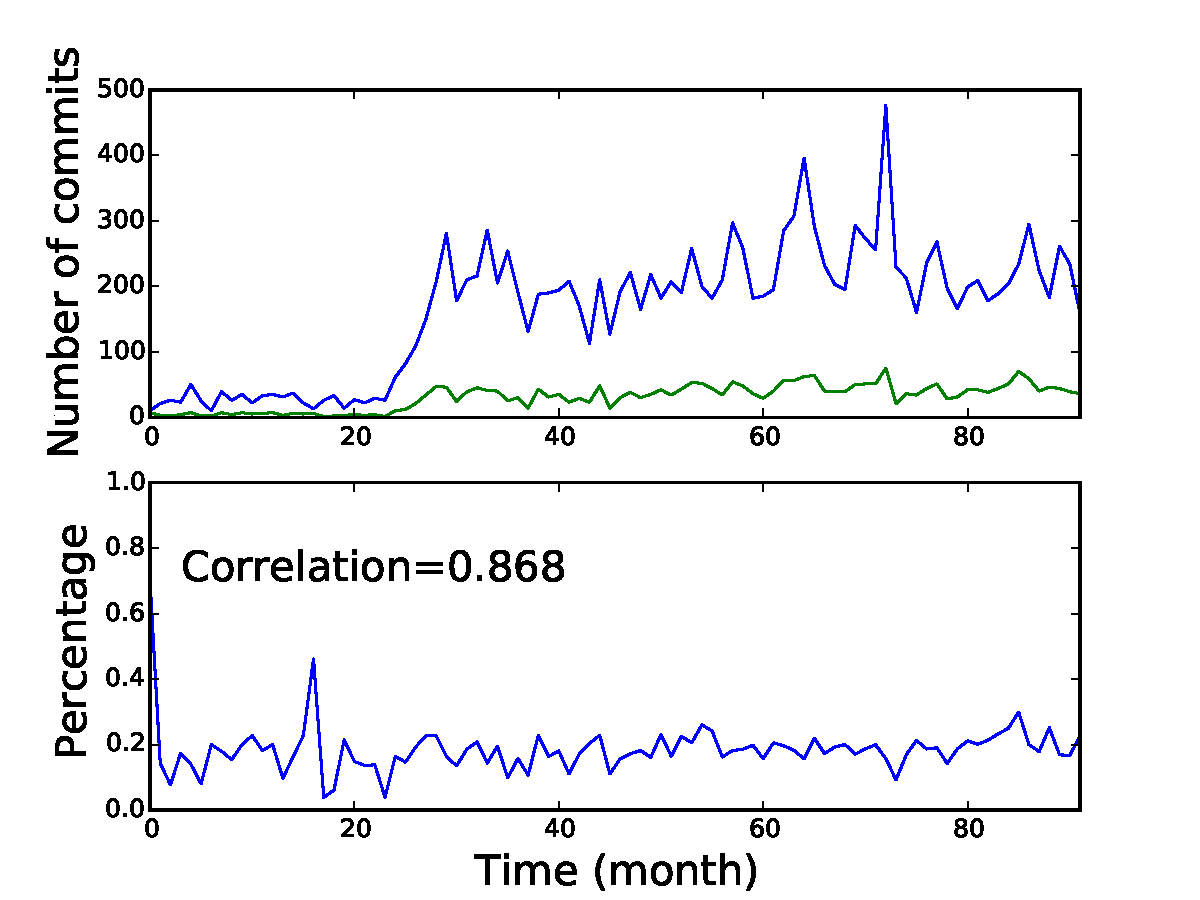
\includegraphics[height=1.4in]{hadoop}}
	\subfigure[Lucene-Solr]{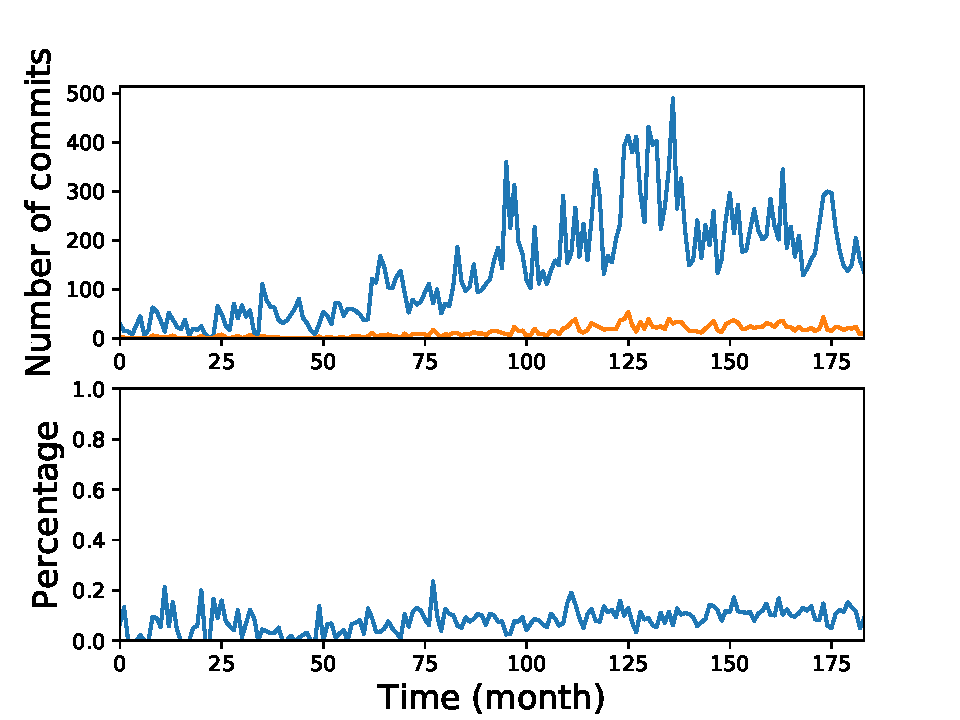
\includegraphics[height=1.4in]{lucene-solr}}
	\subfigure[Netty]{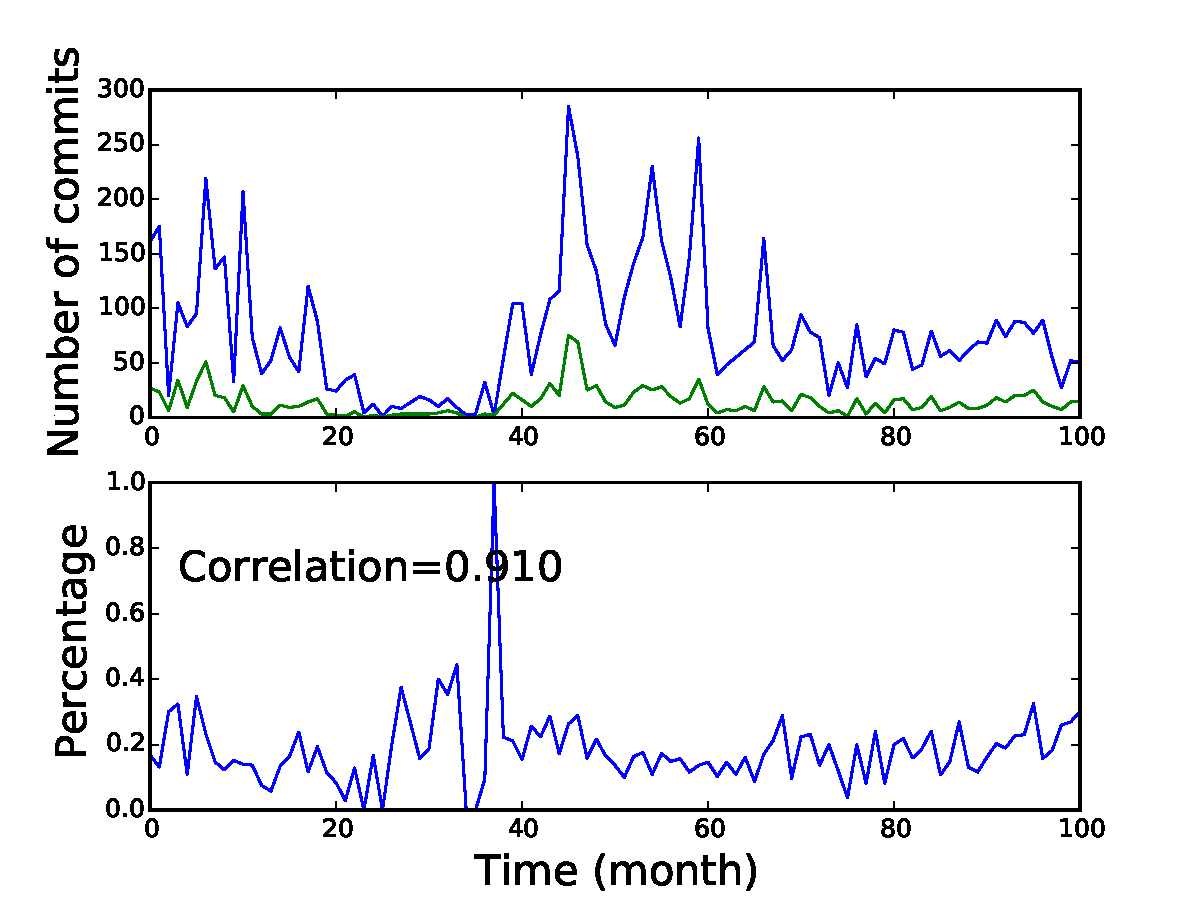
\includegraphics[height=1.4in]{netty}}
	\subfigure[Tomcat]{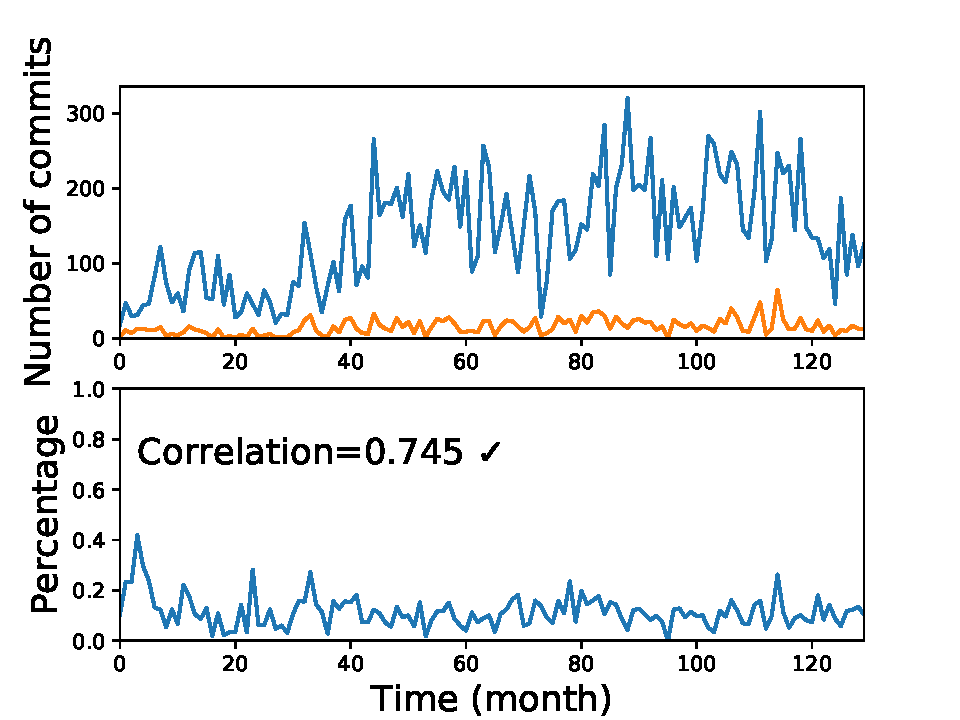
\includegraphics[height=1.4in]{tomcat}}
	\caption{Number of concurrency-related commits compared to all commits}
	\label{fig:confidence}\vspace*{-3ex}
\end{figure*}

This pull request has been accepted.
%However, their programmers denied the pull request. Although our pull request works, it is more neat to systematically replace the above \CodeIn{Counter} class with the \CodeIn{AtomicInteger} class. Their programmers may deny our pull request, simply because the wrapper style looks ugly.

In summary, our results show that our change patterns are repetitive in future maintenance, and programmers confirmed that our change patterns are useful. However, our results also reveal that it needs much programming experience to fully unleash the potential of our change patterns. We further discuss this issue in Section~\ref{sec:discuss}.

\subsection{RQ3. What are the change trends of using parallel APIs}
\label{sec:result:trend}


%\begin{figure}
%	\centering
%	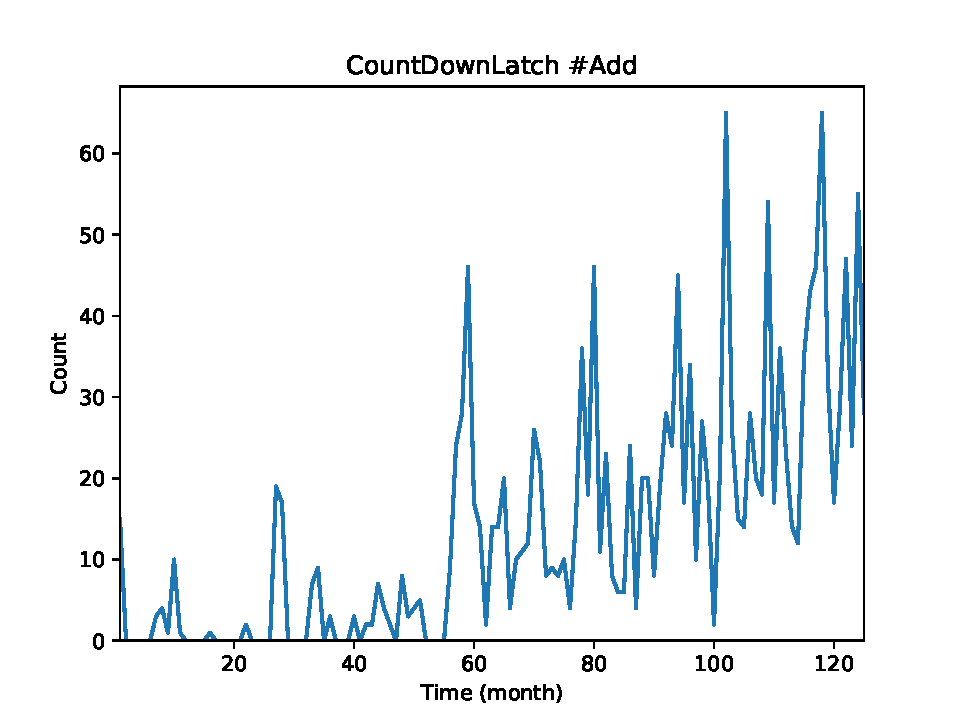
\includegraphics[height=1.5in]{CountDownLatchAdd}
%	\caption{Addition of CountDownLatch}
%\end{figure}
%
%\begin{figure}
%	\centering
%	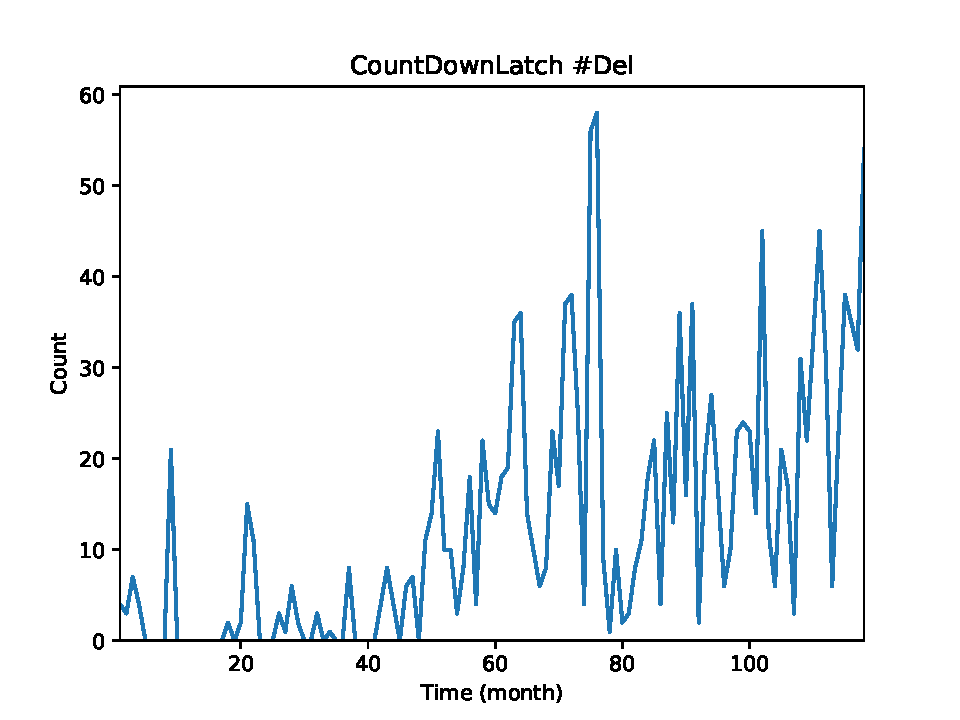
\includegraphics[height=1.5in]{CountDownLatchMinus}
%	\caption{Removal of CountDownLatch}
%\end{figure}
Table~\ref{table:topapi} shows the top ten active parallel API classes in Java. Column ``class'' lists names of these classes. Column ``Occurrence'' lists their occurrences in our concurrency-related commits. Dig~\cite{conf/sigsoft/OkurD12} found that in C\#, 10\% of parallel API classes account for 90\% of API usages. We find that Java follows similar usages patterns as C\#. However, the distribution of Java is not as screwed as C\#. We find that the top \%10 classes account only for about 50\% of the total occurrences, while the bottom \%10 classes account for 0.36\%.

Based on their occurrences, we put the 53 classes into three categories such as \emph{high-frequency}, \emph{medium-frequency} and \emph{low-frequency}, and each category contains roughly the same number of classes. For each category, we further put its classes into three subcategories such as \emph{ascending}, \emph{descending} and \emph{hybrid}. Figure~\ref{figure:trend} shows the results. The percent in each chart is calculated from the classes with the corresponding trend to the total classes. Although most classes are in the hybrid trend, we notice that in the high-frequent category, 15.1\% of classes are in the ascending subcategory. The trend can indicate that about 1/4 parallel API classes in Java standard libraries are becoming more popular.

In summary, we find that Java parallel API classes follow a similar distribution as C\#, but the distribution is less screwed. However, the trends indicate that the distribution can become more like C\#, since popular ones are becoming more popular.

%Figure (a) shows an example of ascending tendency. It is \CodeIn{CountDownLatch}. We are not meaning it is in a strict ascending order. Its overall tendency is rising. Figure (b) shows an example of descending tendency. It is \CodeIn{LinkedTransferQueue}. However, most charts are like figure (c). They are fluctuating without certain ascending or descending tendency. We divide the classes into 3 parts equally and show one class of each part.

% There are 13 ascending charts, 4 descending charts and 36 hybrid charts.

%We write a program to count and analyze concurrent programming classes usage. Table IV shows top 10 classes added and deleted in the history. Some classes are both active in the added and the deleted column like AtomicInteger and CountDownLatch. This is not surprising because a deletion of class does not mean this class is abandoned. This also indicates this class is active. An interesting observation is that deletions appear more than addition.

%We draw line for addition and removal of each class. Figure 3 and figure 4 show examples. We can see that both numbers of addition and removal increase as a whole as time passing by. This indicates that this class is attracting developers' attention.

\subsection{RQ4. The correlations between total commits and concurrency-related commits.}
\label{sec:result:correlation}

Figure~\ref{fig:confidence} shows our results. Each label denotes a project, and has two associated figures. In particular, the upper figure denotes total commits and concurrency-related commits in the interval of months. Its horizontal axis denotes time, and its vertical axis denotes number of commits. Its blue curve denotes total commits, and its yellow curve denotes concurrency-related commits. We find that the curves of total commits and concurrency-related commits are not quite similar. However, the Spearman's rank correlation coefficient shows that in the five out of six projects, the two sets of values are correlated. One exception is Cassandra, where the correlation value is at the border (0.094).

In the lower figures, we calculate the percents from total commits to concurrency-related commits. Although the two sets of data are correlated, we find that their percents are inconstant. In total, about 20\% of total commits are related to concurrency. However, if we make predication based on the percents, the prediction can be unreliable.

In summary, we find that at a coarser granularity, the correlation between total commits and concurrency-related commits still exists with a strong correlation in general.
%\zhong{Delete the following confidences, since you add them in Figure~\ref{fig:confidence} already}.

%\zhong{Introduce your null hypothesis. Introduce how to decide to reject a null hypothesis. That is, introduce how you determine two curves are coefficient.}.



%The coefficients are 0.094 for Cassandra, 0.844 for Flink, 0.868 for Hadoop, 0.896 for Lucene, 0.910 for Netty and 0.745 for Tomcat. Our result is consistent with Gu's result except one project.

%\zhong{Explain whether your results are consistent with Shan Lu or not. }

\subsection{Threats to Validity}

The threats to internal validity include that our tool can omit some concurrency commits. Due to various issues, our tool can fail to identify all concurrency commits. To reduce the threat, we employ both the query-based search and a classifier in our study. The threat could be further reduced by more advanced identification techniques. The threats to internal validity also include obsolete commits. With the rapid development of software, such commits may present obsolete or even wrong usages. To reduce the threat, in our study, we prefer to recent commits. The threats to external validity include our selected projects and programming language. The number of the projects we select is small. They are all Java-based Apache projects. The threat could be reduced by introducing more projects and languages in future work.


%\section{Discussion}
We also have some interesting findings in collecting and analyzing the concurrent related code changes.

(1) Some changes are contrary. Different developers may modify their code in an opposite direction. Here is an example.

\begin{lstlisting}
commit f5fab1f64ba11e04e52bd6251ca62fc854e9578c
Whoops. Fix regression in r1724015.
Code was used although I can't see why a simple AtomicInteger wasn't sufficient.

+    private final AtomicInteger aprPoolDestroyed = new AtomicInteger(0);
-    private static final AtomicIntegerFieldUpdater<OpenSSLContext> DESTROY_UPDATER = AtomicIntegerFieldUpdater.newUpdater(OpenSSLContext.class, "aprPoolDestroyed");
\end{lstlisting}

A previous commit switched to \texttt{AtomicInteger} from \texttt{AtomicIntegerFieldUpdater}. But now this developer reverse the change. In this example, \texttt{AtomicIntegerFieldUpdater} is a class which enables atomic updates to \texttt{volatile} field of classes. We can see that developers in one project may have divergence in a problem.

(2) Developers are using some code-checking tools like FindBugs to help them inspect their code, but sometimes these tools are not enough.

The examples above show that some developers are using code checking tools like FindBugs. Some tools are useful in development environments \cite{conf/oopsla/AyewahPMPZ07}. But these kind of tools don't help developers correct and eliminate the warnings automatically. One developer in Tomcat said "make the volatile anyway so FindBugs doesn't complain" in the commit log. This indicates code checking tools still have room to improve.

This research provides some implications from different kinds of perspectives.

(1) Developers are facing more and more concurrent programming requirements now. But concurrent programming is notoriously error-prone because of the complexity of data synchronization and thread interleaving. Our study gives developers some guidelines of writing concurrent programs. First, use handy concurrent libraries to finish the job instead of rewrite them by yourself unless all the available concurrent libraries cannot satisfy your requirement and you are absolutely confident of your comcurrent programming skills. Using existing libraries allows you to  write less code to finish the same work and enjoy the high quality of implementation which is always reliable, strong and fast. Second, always switch to new-version libraries because they usually provide higher performance and robustness.

(2) Automatic tools are needed to help developers inspect and revise concurrent programs with the help of history information. There has already been some tools, but they usually look for concurrent bugs such as race detection, deadlock detection and atomicity violation without considering software evolution history. Both project specific and project independent transformation patterns exist in real-world software projects. So we need some concurrent code refactoring tools to give advice of what code need change and perform the transformations automatically. It is a chance for IDE manufacturer to make the IDE more intelligent in inspecting and modifying the code. Developers will benefit a lot if such kind of automatic tools can actually help them automate their development and maintaining activities. 
\section{Related work}
\label{sec:related}
\noindent
\textbf{Empirical studies on concurrent programming.} In literature, researchers have conducted various empirical studies to understand concurrent programming. Pinto \emph{et al.}~\cite{journals/jss/PintoTFFB15} conducted a large scale study on the usage of concurrency in Java, and Wu \emph{et al.}~\cite{journals/infsof/WuCZX16} replicated their study with C++. Okur and Dig~\cite{conf/sigsoft/OkurD12} studied how developers use parallel libraries in C\#. David \emph{et al.}~\cite{conf/sosp/DavidGT13} conducted an empirical study to investigate synchronization at both hardware and software levels. Sadowski \emph{et al.}~\cite{conf/msr/SadowskiYK12} studied the evolution of data races, and they found that many data races always exist. Xin \emph{et al.}~\cite{conf/icsm/XinQHXZWG13} conducted an empirical study on lock usage, and they found that most functions acquire only a lock. Lu \emph{et al.}~\cite{conf/asplos/LuPSZ08} studied characteristics of real world concurrency bugs. The above approaches do not analyze change patterns, which are complemented by our study.

%\noindent
%\textbf{Program transformation.} Researchers proposed approaches that transform a source program to its target program. Okur \emph{et al.}~\cite{conf/ecoop/OkurED14} proposed an approach that updates concurrent code with more recent APIs. For Android applications, Lin \emph{et al.}~\cite{conf/sigsoft/LinRD14} proposed an approach that transforms self-written concurrent code to the Android concurrency API, \CodeIn{AsyncTask}. Meng \emph{et al.}~\cite{conf/pldi/MengKM11} proposed an approach that systematically updates code according to given examples. With our findings, it is feasible to implement a tool that further reduces the effort of maintaining concurrent code.

\noindent
\textbf{Identification of commits.} Zhong and Su~\cite{zhong2015bugfix} relied on simple heuristic to identify bug fixes from commits. Tian \emph{et al.}~\cite{tian2012identifying} trained a classifier to identify bug fixes based on their extracted features. Wu \emph{et al.}~\cite{wu2011relink} built the links between bug fixes and their reports based their similarity values. The above approaches focus on identifing bug fixes from commits. In our study, we implement a tool that identifies concurrency-related commits, complementing the above approaches.

\section{Conclusion}
Concurrency programming is challenging, and a mistake can introduce hidden bugs that are difficult to be detected. During software maintenance, programmers have to handle concurrency code carefully. Researchers have conduct various empirical studies to understand concurrency programming. However, how programmers maintain concurrency code is still rarely studied. In this paper, we conduct an empirical study to understand the change patterns and other perspectives of concurrency programming. Based on our analysis results, we summarize five change patterns. We show that such change patterns are repetitive in future maintenance, and programmers have confirmed the usefulness of our extracted patterns. Furthermore, our study comes to other findings such as the trends of parallel API classes and the correlation between total commits and concurrency-related commits, whose usefulness is worthy of further exploration in future work. 








% An example of a floating figure using the graphicx package.
% Note that \label must occur AFTER (or within) \caption.
% For figures, \caption should occur after the \includegraphics.
% Note that IEEEtran v1.7 and later has special internal code that
% is designed to preserve the operation of \label within \caption
% even when the captionsoff option is in effect. However, because
% of issues like this, it may be the safest practice to put all your
% \label just after \caption rather than within \caption{}.
%
% Reminder: the "draftcls" or "draftclsnofoot", not "draft", class
% option should be used if it is desired that the figures are to be
% displayed while in draft mode.
%
%\begin{figure}[!t]
%\centering
%\includegraphics[width=2.5in]{myfigure}
% where an .eps filename suffix will be assumed under latex,
% and a .pdf suffix will be assumed for pdflatex; or what has been declared
% via \DeclareGraphicsExtensions.
%\caption{Simulation results for the network.}
%\label{fig_sim}
%\end{figure}

% Note that the IEEE typically puts floats only at the top, even when this
% results in a large percentage of a column being occupied by floats.


% An example of a double column floating figure using two subfigures.
% (The subfig.sty package must be loaded for this to work.)
% The subfigure \label commands are set within each subfloat command,
% and the \label for the overall figure must come after \caption.
% \hfil is used as a separator to get equal spacing.
% Watch out that the combined width of all the subfigures on a
% line do not exceed the text width or a line break will occur.
%
%\begin{figure*}[!t]
%\centering
%\subfloat[Case I]{\includegraphics[width=2.5in]{box}%
%\label{fig_first_case}}
%\hfil
%\subfloat[Case II]{\includegraphics[width=2.5in]{box}%
%\label{fig_second_case}}
%\caption{Simulation results for the network.}
%\label{fig_sim}
%\end{figure*}
%
% Note that often IEEE papers with subfigures do not employ subfigure
% captions (using the optional argument to \subfloat[]), but instead will
% reference/describe all of them (a), (b), etc., within the main caption.
% Be aware that for subfig.sty to generate the (a), (b), etc., subfigure
% labels, the optional argument to \subfloat must be present. If a
% subcaption is not desired, just leave its contents blank,
% e.g., \subfloat[].


% An example of a floating table. Note that, for IEEE style tables, the
% \caption command should come BEFORE the table and, given that table
% captions serve much like titles, are usually capitalized except for words
% such as a, an, and, as, at, but, by, for, in, nor, of, on, or, the, to
% and up, which are usually not capitalized unless they are the first or
% last word of the caption. Table text will default to \footnotesize as
% the IEEE normally uses this smaller font for tables.
% The \label must come after \caption as always.
%
%\begin{table}[!t]
%% increase table row spacing, adjust to taste
%\renewcommand{\arraystretch}{1.3}
% if using array.sty, it might be a good idea to tweak the value of
% \extrarowheight as needed to properly center the text within the cells
%\caption{An Example of a Table}
%\label{table_example}
%\centering
%% Some packages, such as MDW tools, offer better commands for making tables
%% than the plain LaTeX2e tabular which is used here.
%\begin{tabular}{|c||c|}
%\hline
%One & Two\\
%\hline
%Three & Four\\
%\hline
%\end{tabular}
%\end{table}


% Note that the IEEE does not put floats in the very first column
% - or typically anywhere on the first page for that matter. Also,
% in-text middle ("here") positioning is typically not used, but it
% is allowed and encouraged for Computer Society conferences (but
% not Computer Society journals). Most IEEE journals/conferences use
% top floats exclusively.
% Note that, LaTeX2e, unlike IEEE journals/conferences, places
% footnotes above bottom floats. This can be corrected via the
% \fnbelowfloat command of the stfloats package.




% conference papers do not normally have an appendix


% use section* for acknowledgment
%\section*{Acknowledgment}

%The authors would like to thank my mentor and anyone who might have helped us with this study.



% trigger a \newpage just before the given reference
% number - used to balance the columns on the last page
% adjust value as needed - may need to be readjusted if
% the document is modified later
%\IEEEtriggeratref{8}
% The "triggered" command can be changed if desired:
%\IEEEtriggercmd{\enlargethispage{-5in}}

% references section

% can use a bibliography generated by BibTeX as a .bbl file
% BibTeX documentation can be easily obtained at:
% http://mirror.ctan.org/biblio/bibtex/contrib/doc/
% The IEEEtran BibTeX style support page is at:
% http://www.michaelshell.org/tex/ieeetran/bibtex/
\balance
\bibliographystyle{abbrv}
% argument is your BibTeX string definitions and bibliography database(s)
\bibliography{bare_conf}
%
% <OR> manually copy in the resultant .bbl file
% set second argument of \begin to the number of references
% (used to reserve space for the reference number labels box)
%\begin{thebibliography}{1}
%
%\bibitem{IEEEhowto:kopka}
%H.~Kopka and P.~W. Daly, \emph{A Guide to \LaTeX}, 3rd~ed.\hskip 1em plus
%  0.5em minus 0.4em\relax Harlow, England: Addison-Wesley, 1999.
%
%\end{thebibliography}




% that's all folks
\end{document}


